\documentclass[journal]{IEEEtran}

% ===== 中文支持 =====
\usepackage[UTF8]{ctex}

% ===== 常用宏包 =====
\usepackage{cite}
\usepackage{amsmath,amssymb,amsfonts}
\usepackage{textcomp}
\usepackage{graphicx}
\usepackage{tabularx}
\usepackage[colorlinks=true, allcolors=blue]{hyperref}
\usepackage[ruled,vlined,linesnumbered]{algorithm2e}
\usepackage{float}
\usepackage[font=footnotesize]{caption}
\usepackage{subcaption}
\usepackage{tikz}
\usetikzlibrary{
    shapes.geometric,
    shapes,
    arrows.meta,
    positioning,
    fit,
    calc
}
\usepackage{amsthm}

% ===== 中文图表/算法/定理环境 =====
\renewcommand{\figurename}{图}
\renewcommand{\tablename}{表}
\renewcommand{\refname}{参考文献}
\renewcommand{\appendixname}{附录}
\renewcommand{\algorithmcfname}{算法}
\renewcommand{\listalgorithmcfname}{算法目录}

\theoremstyle{plain}
\newtheorem{theorem}{定理}
\newtheorem{proposition}{命题}
\newtheorem{lemma}{引理}
\newtheorem{corollary}{推论}
\theoremstyle{definition}
\newtheorem{remark}{注}
\renewcommand{\qedsymbol}{$\blacksquare$}

\begin{document}

% ===== 标题 =====
\title{面向网络韧性治理的系统弛豫机制：一种对抗结构应力集中的模型驱动控制方法}

\author{Jie~Ding,
       Zhiyuan~Ren,~\IEEEmembership{Member,~IEEE},
       Wenchi~Cheng,~\IEEEmembership{Senior~Member,~IEEE},
       and~Zhiliang Shuai
\thanks{本工作得到多域数据协同处理与控制全国重点实验室开放基金资助（No. MDCPC-20250108）。}
\thanks{Jie Ding 就职于多域数据协同处理与控制全国重点实验室，北京市丰台区大成路13号。}
\thanks{Zhiyuan Ren、Wenchi Cheng 和 Zhiliang Shuai 就职于西安电子科技大学通信工程学院，西安 710071。}
\thanks{通信作者：Zhiyuan Ren（zyren@xidian.edu.cn）。}
}

\maketitle

% ===== 摘要 =====
\begin{abstract}
当前主流网络控制策略大多建立在静态最短路径逻辑之上，天然存在“应力集中”问题：流量会过度汇聚到少数关键节点，从而引发结构脆弱性并导致容量提前饱和。尽管现有面向负载或基于人工智能的方法试图通过反应式选路来缓解拥塞，但由于忽略了对网络代价地形的主动调控，它们并未触及问题的结构性根源。为此，本文提出系统弛豫算法（System Relaxation Algorithm, SRA），这是一种受物理弛豫过程启发的模型驱动型监督治理层，能够引导网络向负载均衡的“弛豫平衡态”演化。SRA 是一个可解释的“白盒”动力系统，其中节点代价依据历史累积的结构应力持续演化。通过将离散路径切换建模为非光滑动力系统，本文利用分段 Lyapunov 函数严格证明了系统的全局收敛性与实用稳定性，并揭示传统静态路由实际上只是该更一般框架中“阻尼消失”的退化无记忆情形。大量仿真表明，SRA 的行为强烈依赖于网络拓扑：在异质网络中，它表现为一种主动性能优化器，峰值中心性可降低 80\% 以上，吞吐量提升超过 45\%；而在同质拓扑中，它会智能地将优化目标转向韧性增强。由此，SRA 为网络治理建立了一种可预测、可数学分析的新范式，能够在性能与韧性之间实现具有拓扑感知能力的智能权衡。
\end{abstract}

\begin{IEEEkeywords}
网络控制，应力感知治理，网络韧性，自组织系统，负载均衡，非光滑动力系统，稳定性分析。
\end{IEEEkeywords}

% ===== 正文 =====
\section{引言}
\label{sec:introduction}

\IEEEPARstart{现}{代}通信网络——从数据中心网络到大规模运营商骨干网——都运行在高度波动的业务环境中，因此系统稳定性至关重要。
在这类高风险场景下，建立在静态最短路径逻辑上的主流网络控制范式正面临根本性危机。
这类传统协议天然缺乏管理结构应力的机制，从而导致本文所称的“应力集中”现象：负载会不成比例地汇聚到少数关键拓扑瓶颈节点。
这不仅仅是瞬时拥塞问题，更是一种结构性脆弱性：它会制造“应力奇点”，使网络更容易遭受级联失效；同时还会导致容量提前饱和，即网络在尚未达到物理极限容量之前，瓶颈位置就已出现大规模丢包与时延急剧上升。

\begin{figure}[t!]
    \centering
    \begin{subfigure}[b]{0.47\columnwidth}
        \centering
        \begin{tikzpicture}[scale=0.85]
            \tikzstyle{node}=[circle, draw, thick, minimum size=6mm]
            \tikzstyle{hub}=[node, fill=red!80, minimum size=10mm]
            \tikzstyle{flow}=[-Latex, gray, thick, shorten <=1mm, shorten >=1mm]
            \node[hub] (H) at (0,0) {};
            \node[node] (N1) at (2,1) {};
            \node[node] (N2) at (2,-1) {};
            \node[node] (N3) at (-2,1.5) {};
            \node[node] (N4) at (-2,-1.5) {};
            \node[node] (P1) at (0, 2.2) {};
            \node[node] (P2) at (0, -2.2) {};
            \draw (H) -- (N1); \draw (H) -- (N2);
            \draw (H) -- (N3); \draw (H) -- (N4);
            \draw (H) -- (P1); \draw (H) -- (P2);
            \draw[flow, line width=1.2pt] (N3) to [bend left=10] (H);
            \draw[flow, line width=1.2pt] (N4) to [bend right=10] (H);
            \draw[flow, line width=1.2pt] (H) to [bend left=10] (N1);
            \draw[flow, line width=1.2pt] (H) to [bend right=10] (N2);
            \node[below=0.1cm of H, text=red!80!black, font=\bfseries] {应力奇点};
        \end{tikzpicture}
        \caption{传统范式：应力集中}
        \label{fig:intro_before}
    \end{subfigure}
    \hfill
    \begin{subfigure}[b]{0.47\columnwidth}
        \centering
        \begin{tikzpicture}[scale=0.85]
            \tikzstyle{node}=[circle, draw, thick, minimum size=6mm]
            \tikzstyle{hub}=[node, fill=yellow!80, minimum size=8mm]
            \tikzstyle{periph}=[node, fill=green!20]
            \tikzstyle{flow}=[-Latex, green!50!black, thick, shorten <=1mm, shorten >=1mm]
            \node[hub] (H) at (0,0) {};
            \node[periph] (N1) at (2,1) {};
            \node[node] (N2) at (2,-1) {};
            \node[periph] (N3) at (-2,1.5) {};
            \node[node] (N4) at (-2,-1.5) {};
            \node[periph] (P1) at (0, 2.2) {};
            \node[node] (P2) at (0, -2.2) {};
            \draw (H) -- (N1); \draw (H) -- (N2);
            \draw (H) -- (N3); \draw (H) -- (N4);
            \draw (H) -- (P1); \draw (H) -- (P2);
            \draw[flow, line width=1.2pt] (N3) to [bend left=40] (P1);
            \draw[flow, line width=1.2pt] (P1) to [bend left=40] (N1);
            \draw[flow, line width=1.2pt] (N1) to [bend right=40] (N2);
            \node[below=0.1cm of H, text=green!60!black, font=\bfseries] {应力分散};
        \end{tikzpicture}
        \caption{SRA 控制范式：系统弛豫}
        \label{fig:intro_after}
    \end{subfigure}

    \caption{核心问题与本文所提 SRA 范式的概念示意图。SRA 通过引导系统进入负载更加均衡的“弛豫状态”，缓解传统网络控制中固有的“应力集中”问题。}
    \vspace{-4mm}
    \label{fig:intro_scenario}
\end{figure}

这种脆弱性的根源在于：现有方法关注的是拥塞症状的被动响应，而不是结构压力的主动治理。
既有工作主要试图从以下两条路径修补这一问题，但都没有触及结构性成因：
\begin{itemize}
    \item \textbf{反应式负载感知路由（如 \cite{Macabale2020Cradle}）：} 这类方法根据队列长度等瞬时指标调整路径，本质上是一种“对症处理”。在高负载场景中，由于反馈滞后，系统容易发生振荡。
    \item \textbf{黑盒式 AI 控制（如 \cite{Wei2023GRLPS}）：} 深度强化学习方法虽可隐式学习拓扑特征，但其决策过程不可解释，难以为关键基础设施提供安全性保障。
\end{itemize}

如表~\ref{tab:related_work_comparison} 所示，现有方案并未真正将结构应力与瞬时流量状态解耦。
它们关注的是在既定代价地形上的“寻路”，而问题的根本解法应当是主动“调控地形本身”。

为弥补这一空缺，本文借鉴物理系统中的“弛豫”思想，将研究视角从被动寻路转向主动的\textit{结构应力治理}。
我们提出系统弛豫算法（SRA），它通过动态重塑网络的代价地形来分散结构应力。
不同于黑盒方法，SRA 是一个可解释的白盒动力系统：它通过“泄漏积分器”机制把历史应力累积为一个可控状态变量，进而引导网络自发演化到一种负载均衡的平衡态（概念上如图~\ref{fig:intro_scenario} 所示）。
更重要的是，该控制范式天然契合软件定义网络（SDN）架构：控制器利用其全局视图计算应力状态，并凭借集中控制能力下发相应的代价策略。

\begin{table*}[h!]
\centering
\caption{网络控制范式的分类与比较}
\label{tab:related_work_comparison}
\renewcommand{\arraystretch}{1.3}
\small
\begin{tabularx}{\textwidth}{|l|X|X|X|X|}
\hline
\textbf{特征} & \textbf{反应式负载感知} & \textbf{静态结构优化} & \textbf{AI 驱动 / 学习式控制} & \textbf{SRA（本文）} \\
\hline \hline
\textbf{感知对象} & 瞬时流量状态（如队列长度、丢包） & 静态图指标（如 BC、度） & 高维模式与图结构特征 & \textbf{累积结构应力（$S$）} \\
\hline
\textbf{控制逻辑} & 对瞬时扰动的对症反应 & 固定权重上的开环寻路 & 黑盒策略逼近（RL/GNN） & \textbf{闭环模型驱动动力学} \\
\hline
\textbf{数学基础} & 启发式代价函数 & 图论与优化 & 统计学习与推断 & \textbf{非光滑动力系统} \\
\hline
\textbf{稳定性保证} & 无（易振荡、易出现乒乓） & 不适用（静态/开环） & 经验性（难以给出 Lyapunov 证明） & \textbf{严格可证（全局吸引性与 Lyapunov 衰减）} \\
\hline
\textbf{主要目标} & 缓解局部短时拥塞 & 面向平均场景的结构优化 & 最大化特定 KPI（吞吐/时延） & \textbf{分散内生结构应力} \\
\hline
\textbf{部署方式} & 本地 / 分布式 & 集中式（离线） & 集中式（高算力训练） & \textbf{兼容 SDN（模型驱动）} \\
\hline
\textbf{可解释性} & 高 & 高 & 低 & \textbf{高（白盒控制律）} \\
\hline
\end{tabularx}
\end{table*}

本文的主要贡献如下：
\begin{enumerate}
    \item \textbf{统一的控制论框架：} 我们将结构应力（以介数中心性表征）形式化为闭环动力系统中的可控状态变量。该框架明确地将结构应力治理与底层选路过程解耦，并把传统静态路由视为当系统记忆保持项取零时的一个退化特例。
    \item \textbf{对不连续动力学的严格分析：} 本文首次将基于中心性的离散路径切换建模为\textit{非光滑动力系统}。借助微分包含理论与分段 Lyapunov 函数，我们严格证明了系统的全局收敛性与实用稳定性，从而避免了启发式自适应路由常见的破坏性振荡。
    \item \textbf{拓扑相关的智能性：} 大量仿真表明，SRA 在不同拓扑中会涌现出不同角色：在异质网络（如无标度网络）中，它表现为\textit{性能优化器}，通过抑制瓶颈提升吞吐；在同质网络（如随机图）中，它则自动转化为\textit{韧性增强机制}，以极小的时延代价换取更稳定的分组投递能力。
\end{enumerate}

本文聚焦于应力感知网络治理的算法基础与稳定性分析。
尽管我们讨论了其与 SDN 架构的契合关系，但具体硬件实现及南向协议扩展不在本文讨论范围之内。
后续内容安排如下：第~\ref{sec:related_work} 节对相关工作进行分类并定位 SRA 所处的研究位置；第~\ref{sec:model} 节建立统一理论框架，包括控制模型、基于非光滑动力学的稳定性分析，以及与容量扩展之间的理论桥接；第~\ref{sec:simulation} 节给出跨拓扑仿真验证与分析；第~\ref{sec:discussion_conclusion} 节总结全文。

\section{相关工作}
\label{sec:related_work}

结构应力的缓解问题始终是网络科学与流量工程交叉领域中的核心挑战。
现有方法虽然都试图改进流量分布均衡性，但它们对“网络状态”的理解方式及相应控制机制存在显著差异。
如表~\ref{tab:related_work_comparison} 所总结，传统“寻路”策略与主动“重塑代价地形”之间存在清晰鸿沟。
为了将本文提出的系统弛豫算法（SRA）放到更广泛的研究背景下，我们把现有工作划分为三类：反应式对症管理、静态结构优化，以及黑盒学习式控制。

\subsection{反应式控制：对症缓解及其局限}

网络控制中最常见的范式，是依据实时性能指标通过\textit{反应式}反馈回路调整路径。
这类协议通常监测本地队列长度 \cite{Macabale2020Cradle}、能量感知型负载指标 \cite{SM2025Novel}，或在高动态卫星与车联网环境中的复合链路质量 \cite{Wang2025VANET, Fu2024SatelliteBC}。
例如，CRADLE 协议 \cite{Macabale2020Cradle} 利用跨层信息引导流量偏转；多准则决策模型 \cite{Fouad2014MultiCriteria} 与分层聚类扩展方法 \cite{Guizani2011Hierarchical} 则尝试在需求波动场景下优化路由决策。
近年来在物联网和智慧城市领域的研究，进一步把这一思路推广到位置驱动和遮挡驱动的路由 \cite{Darabkh2025SmartCity, Aditya2020ClosenessCluster}，以应对高速传输节点中常见的级联时延问题 \cite{Wu2024RailwayNode}。

尽管这些方法在缓解即时拥塞方面有效，但它们本质上仍是“症状缓解器”，处理的是缓存溢出或链路饱和等表层现象，而不是其背后的\textit{结构性根源}。
由于把网络代价地形视为不可改变的外在约束，反应式方法只能被动追随瞬时流量扰动。
因此，它们极易受到“乒乓效应”的影响：路径会在过载和欠载状态之间来回摆动。
由于缺乏 SRA 中那种长期积分与泄漏记忆机制，这些方法无法区分瞬时流量尖峰和内生结构应力，也缺乏足够严格的数学框架来保证在非光滑流量动态下的全局稳定性。

\subsection{静态结构优化：开环治理缺口}

考虑到网络拓扑的决定性作用，大量研究利用中心性指标来指导路由和资源分配。
介数中心性（BC）及其扩展形式——例如面向光网络的链路方差优化 \cite{Upadhyay2024OpticalBC}、面向复用系统的加权引力模型 \cite{Ni2023Gravity}——已成为识别拓扑瓶颈和关键节点的重要手段 \cite{Basaras2019Influential, Wehmuth2021SpuriousPaths}。
相关理论进一步指出，通过准最短路径（$\rho$-测地线） \cite{DeMedeiros2017QuasiShortest} 或在概率失效模型下优化连通性 \cite{Cavallaro2022Connectivity}，可以显著增强网络韧性。
为了降低全局中心性分析固有的 $O(N^3)$ 复杂度，近年来又提出了多种高效近似方法，包括双曲空间嵌入 \cite{Stai2017Hyperbolic}、聚类并行化 \cite{Suppa2015FastBC} 和分布式估计框架 \cite{Maccari2020DistributedLoad, Maccari2018DistributedDV}。
这些结构性分析已被应用于诸多场景，如优化 SDN 流表存储 \cite{Ma2019FlowTable}、支持稀疏网络中的贪婪转发 \cite{Ahmed2025SparseNet} 以及无线传感器网络中的节能路径规划 \cite{Oliveira2010WSNcentrality}。

然而，这类结构优化方法从根本上说仍然是\textit{开环}且描述性的。
即便考虑中心性的时间变化 \cite{Ghanem2019DynamicCentrality}，相关指标也只是被动观测量，而不是可被控制的系统状态。
这类策略通常针对静态或平均意义下的拓扑进行优化，无法刻画真实流量与拓扑约束耦合后产生的非线性“压力积累”过程。
与 SRA 不同，它们缺少一种严格的控制律，无法把结构观测映射为可自适应调节的代价地形，从而在“拓扑感知”与“主动抑制拥塞”之间留下了明显的治理鸿沟。

\subsection{AI 驱动与自组织控制：黑盒困境}

近年来机器学习的迅速发展，推动了深度强化学习（DRL）和图神经网络（GNN）在复杂网络管理中的应用。
例如 GRL-PS \cite{Wei2023GRLPS} 和多智能体 GNN 框架 \cite{Feng2025MultiAgentGNN}，都试图通过隐式学习拓扑特征来应对复杂拥塞场景。
为了减少全局中心性计算开销，还有研究借助节点嵌入来近似传统中心性度量 \cite{Mendonca2021ApproxCentrality}。
与此同时，受生物启发的自组织模型 \cite{Cheng2010SelfOrganizingModel, Guo2010HybridSelfOrg, Li2014PhysarumMulticast}，以及离散粒子群优化 \cite{Wang2019DPSO}、遗传算法 \cite{Mu2024CarrierSelfOrg} 等启发式搜索方法，也被用于动态簇式路由场景。
这类自主寻路能力在导弹蜂群网络等任务关键型场景中尤受关注，因为节点必须适应快速变化的拓扑 \cite{Lu2022MissileSwarm}。

然而，这些方法虽然在经验上表现良好，却往往是\textit{黑盒}系统，其决策逻辑缺乏透明性。
它们通常无法提供形式化安全验证，也难以给出严格的 Lyapunov 稳定性保证；而在关键基础设施环境中，DRL 智能体的不可预测收敛性本身就是一种系统性风险。
此外，启发式与自组织模型通常忽略了离散路径切换所带来的内在非光滑不连续性。
SRA 则通过严格引入非光滑动力系统理论，提供了一种“白盒”替代方案，从而同时实现数学可解释性与全局收敛保证。

总的来看，上述三类方法都推动了网络工程的发展，但“拓扑感知”与“主动治理”之间的关键缺口依然存在。
反应式方法追求速度而牺牲稳定性；静态结构优化虽具诊断深度，却缺少执行机制；学习式控制则以数学可解释性的损失换取经验性能。
尤其是，当前网络研究仍缺乏一个统一框架，能够把高层结构观测（如中心性）与具备全局稳定性保证的底层流量控制律有效衔接起来。
本文提出的系统弛豫算法（SRA）正是为填补这一缺口而设计：它以非光滑动力系统理论和“代价律”为基础，把网络管理思想从被动寻路推进到主动、稳定、可解释的代价地形重塑。

% ===== 后续章节请继续沿用同样方式翻译 =====
\section{理论模型与方法}
\label{sec:model}

我们并不将面向结构应力治理的网络控制问题表述为一系列启发式路由更新，而是将其形式化为一个\textbf{离散时间、非光滑动力系统}。
这种控制论视角是关键的：它使我们能够超越朴素反应式协议常见的稳定性陷阱，因为后者由于缺乏系统记忆，往往会退化为破坏性的持续振荡。
在我们的框架中，网络的代价地形不再是静态输入，而是由一种受物理系统启发的“泄漏积分器”所驱动的动态状态变量。
本节系统地构建这一模型。
我们首先定义网络模型，并将结构应力形式化为可控状态；随后给出将连续压力积累与离散路径切换耦合起来的核心状态演化规律；最后，借助分段 Lyapunov 函数与离散时间包含系统理论，严格证明 SRA 能够全局收敛到一个鲁棒平衡状态——这是启发式方法根本无法提供的理论保证。

\subsection{网络模型与负载度量}

我们将底层网络拓扑建模为一个连通无向图 $G=(V,E)$，其中节点数为 $N=|V| \ge 3$。
从控制系统的角度看，网络这一“被控对象”由一个动态演化的节点代价向量 $C \in \mathbb{R}^N_+$ 所支配。
该向量定义了瞬时\textit{代价地形}：任一路径 $P$ 的代价为其所经过节点的转发代价之和，即
$d(P) = \sum_{v \in P} C_v$。
假定业务流总是沿当前代价地形下的最低代价路径进行转发。

为刻画给定代价分布所诱导的结构应力，我们采用\textbf{介数中心性（Betweenness Centrality, BC）}作为主要反馈信号。
节点 $i$ 上的未归一化应力，记为 $\kappa_i(S)$，表示其所承受的绝对拓扑负载：
\begin{equation}
    \label{eq:bc_definition}
    \kappa_i(S) = \sum_{s\neq i\neq t\in V} \frac{\sigma^{\,C(S)}_{st}(i)}{\sigma^{\,C(S)}_{st}}
\end{equation}
其中，$\sigma^{\,C(S)}_{st}$ 表示在代价配置 $C(S)$ 下，节点对 $(s,t)$ 之间最短路径的总数，$\sigma^{\,C(S)}_{st}(i)$ 则表示其中经过节点 $i$ 的那一部分。

由于 $\kappa_i(S)$ 是无界的，我们将该反馈信号投影到紧致状态空间中，以保证系统稳定。
定义最大值归一化后的应力向量为：
\begin{equation}
    \label{eq:bc_normalization}
    \mathrm{norm}(\kappa(S)) :=
    \begin{cases}
    \displaystyle \frac{\kappa(S)}{\max_{j}\kappa_j(S)}, & \text{if } \max_j \kappa_j(S) > 0,\\[6pt]
    \mathbf{0}, & \text{otherwise.}
    \end{cases}
\end{equation}
这一归一化将反馈信号严格约束在单位超立方体 $[0,1]^N$ 内。

\textbf{关键几何性质：}
更关键的是，对于任意有限图，在采用确定性并列路径裁决规则时，所有可能的最短路径配置集合是有限的。
这意味着 $\mathrm{norm}(\kappa(S))$ 并不是连续变化的，而是在一个\textbf{有限个常向量组成的集合}之间跳变。
这一量化特性并非细枝末节；恰恰相反，它使得系统动力学成为\textit{分段常值}的，从而构成了第~\ref{sec:convergence_analysis} 节中非光滑收敛性分析的拓扑基础。

\begin{figure*}[t!]
    \centering
    \begin{tikzpicture}[
        auto,
        node distance=1.5cm and 2.5cm,
        plant/.style={rectangle, draw, fill=blue!10, text width=10em, text centered, rounded corners, minimum height=5em},
        module/.style={rectangle, draw, fill=green!10, rounded corners, text width=8em, text centered, minimum height=4em},
        line/.style={draw, -{Latex}},
        signal/.style={draw, -{Latex}, thick},
        feedback/.style={draw, -{Latex}, dashed}
    ]
    % SRA Controller's Internal Modules
    \node [module] (sensing) {感知模块 \\ (\textit{中心性计算})};
    \node [module, right=of sensing] (law) {控制律 \\ (\textit{泄漏积分器})};
    \node [module, right=of law] (actuation) {控制信号生成模块};
    % Network Plant
    \node [plant, below=of law] (plant) {网络被控对象 \\ (\textit{节点、链路、底层路由协议})};
    % Dashed container for the SRA controller
    \node [draw, rounded corners, fit=(sensing) (law) (actuation), label={[yshift=0.2cm]above:\textbf{SRA 控制器}}, inner sep=0.6cm, dashed] (controller_box) {};
    % Connections
    \path [signal] (actuation.south) -- node [right, pos=0.25, align=center] {控制信号 \\ $C^{(k+1)}$（节点代价）} (plant.east);
    \path [feedback] (plant.west) -| node [left, pos=0.25, align=center] {状态反馈 \\ （拓扑、路径）} (sensing.south);
    % Internal Controller Connections
    \path [line] (sensing.east) -- node [above, align=center] {应力 \\ $\kappa^{(k)}$} (law.west);
    \path [line] (law.east) -- node [above, align=center] {压力 \\ $S^{(k+1)}$} (actuation.west);
    % System Performance Output
    \coordinate[right=of plant] (output_coord);
    \path [signal] (plant.east) -- node [right, pos=0.8, align=center] {系统性能 \\ （吞吐量、时延等）} (output_coord);
    \end{tikzpicture}
    \caption{SRA 作为闭环控制系统的体系结构。SRA 控制器充当上层监督治理模块，通过动态调节网络代价地形来治理底层网络被控对象。}
    \label{fig:sra_architecture}
\end{figure*}

\subsection{SRA：核心机制与算法实现}
\label{subsec:sra_mechanism}

\textit{设计理念：SRA 作为监督治理层。}
需要特别强调的是，SRA 并不是一个直接承担分组转发功能的路由协议；相反，它是一个用于优化网络“代价地形”的上层监督治理层。
它为标准路由协议（如 OSPF、IS-IS 或 Dijkstra）提供一个自适应的度量空间，使这些底层协议能够在不触发结构性瓶颈的前提下完成路径计算。

在定义状态空间之后，我们进一步推导 SRA 控制器的\textit{运动规律}。
我们并不只是把 SRA 视作一个路由算法，而是将其严格构造为一个\textbf{闭环反馈控制系统}，其结构如图~\ref{fig:sra_architecture} 所示。
其核心设计思想是：将应力的瞬时观测与代价的即时执行解耦。
具体而言，我们在感知与执行之间插入一个时间积分阶段，也就是一个\textbf{泄漏积分器}，以便 SRA 控制器能够以带阻尼的方式治理底层网络被控对象。
这一设计使 SRA 从根本上区别于那类“失忆式”的反应式协议：它能够滤除高频瞬态扰动，只对持续存在的结构趋势作出响应。

一个朴素的反馈机制若直接将节点代价设置为瞬时中心性的函数，其本质上是不稳定的，因为这会形成一种“bang-bang”式控制，最终导致持续且具有破坏性的振荡。
为了获得严格稳定性，SRA 的设计必须内建系统记忆，以抑制这些高频波动。
我们通过积分（I）控制结构来实现这一点，并将其具体实现为一个\textbf{泄漏积分器}。
定义一个核心状态向量——“累积压力” $S \in \mathbb{R}^N_+$——用以表示每个节点历史积分意义下的应力。
其演化满足如下离散时间状态转移方程：
\begin{equation}
    \label{eq:pressure_update}
    S_i^{(k+1)} = (1 - \alpha) S_i^{(k)} + \alpha \cdot \mathrm{norm}(\kappa_i^{(k)})
\end{equation}
其中，$k$ 为迭代步，学习率 $\alpha \in (0,1)$ 控制系统记忆的保持程度。
从物理上看，该方程相当于一个\textbf{数字低通滤波器}：其中 $(1-\alpha)$ 项提供关键的\textbf{阻尼}效应，使系统既能吸收瞬态流量冲击，又能持续跟踪长期存在的结构趋势。

\begin{remark}[与反应式路由的关系]
\label{rem:reactive_routing}
必须指出，标准反应式路由协议对应于式~\eqref{eq:pressure_update} 的一个\textit{退化情形}，即 $\alpha=1$。
\end{remark}

在这一无记忆极限下，阻尼项消失（$1-\alpha=0$），这也解释了为何此类协议在高负载下天然缺乏稳定性。

随后，节点转发代价 $C$，也就是系统的执行信号，被定义为基于这一稳定历史状态的仿射控制律：
\begin{equation}
    \label{eq:cost_update}
    C_i^{(k+1)} = 1 + \beta_I \cdot S_i^{(k+1)}
\end{equation}
其中，$1$ 表示基础物理代价，$\beta_I > 0$ 为“压力到代价”的增益因子。
由于代价来自系统历史状态 $S$，而非瞬时噪声，因此 SRA 能够作出稳定且具有前瞻性的控制决策。

\begin{figure}[hbtp]
    \centering
    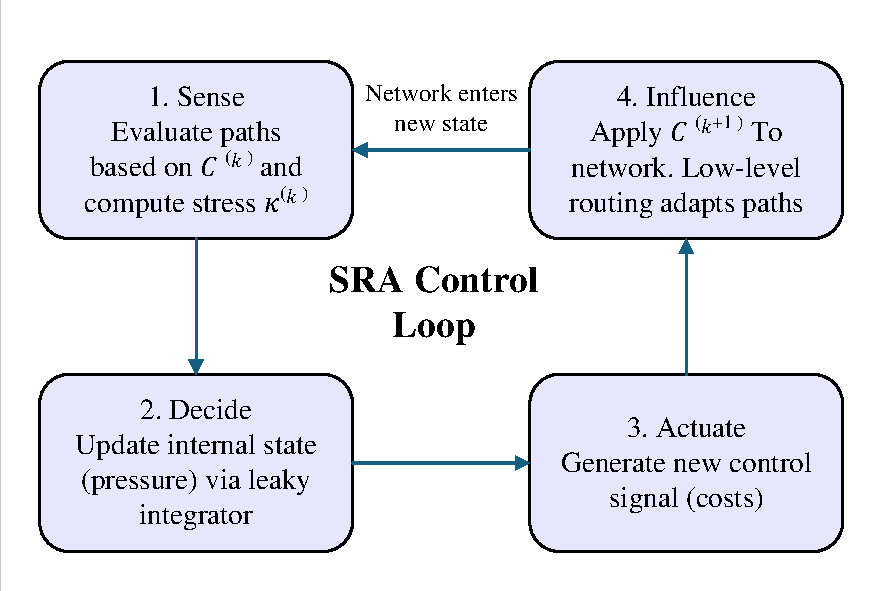
\includegraphics[width=0.9\columnwidth]{fig3xunhuan.pdf}
    \caption{SRA 控制闭环的迭代流程，展示了感知、决策、执行和系统作用四个关键阶段，这些阶段共同驱动网络朝着结构应力分散的状态演化。}
    \label{fig:sra_workflow}
\end{figure}

完整的迭代过程在算法~\ref{alg:sra} 中形式化给出，其循环工作流如图~\ref{fig:sra_workflow} 所示。
为了处理离散路径切换所带来的非光滑性，算法进一步引入了一个\textit{稳定化约束}：最小驻留时间 $T_d$。
这一机制避免系统对其自身控制动作所引起的即时扰动过度响应，从而允许网络状态在下一次更新之前先充分沉降。
SRA 的核心原则是根据累积结构应力，从根本上重塑网络的“代价地形”。
如图~\ref{fig:sra_mechanism_visualization} 的概念示意所示，这一机制迫使路由协议在“路径效率”和“瓶颈规避”之间进行智能权衡，将业务从高应力的短路径引导到更长但更稳定的外围路径上。

\begin{algorithm}[h!]
    \DontPrintSemicolon
    \KwIn{图 $G=(V,E)$；学习率 $\alpha \in (0,1)$；压力代价因子 $\beta_I > 0$；停止阈值 $\varepsilon > 0$；最大迭代次数 $K_{\max}$；（可选）最小驻留时间 $T_d \ge 1$.}
    \KwOut{最终节点代价向量 $C^{(k+1)}$ 及其对应的路由策略。}
    \BlankLine
    \textbf{初始化：} $S^{(0)} \leftarrow \mathbf{0}$；$C^{(0)} \leftarrow \mathbf{1}$\;
    \BlankLine
    \For{$k=0, 1, 2, \dots, K_{\max}-1$}{
        \tcp{步骤1：路径评估}
        基于节点代价 $C^{(k)}$ 计算全对最短路径\;
        \tcp{步骤2：中心性计算}
        根据新路径计算未归一化中心性 $\kappa^{(k)}$\;
        \tcp{步骤3：压力更新}
        $S^{(k+1)} \leftarrow (1-\alpha)S^{(k)}+\alpha\,\mathrm{norm}(\kappa^{(k)})$\;
        \tcp{步骤4：代价更新}
        $C^{(k+1)} \leftarrow 1+\beta_I\,S^{(k+1)}$\;
        \tcp{步骤5：防抖振策略}
        \If{在第 $k$ 步发生了路径集合切换且 $T_d > 1$}{
            接下来强制使用当前路径集合持续 $T_d-1$ 步，仅执行步骤2-6\;
        }
        \tcp{步骤6：收敛判定}
        \If{$\|S^{(k+1)}-S^{(k)}\|_\infty \le \varepsilon$ 且路径集合稳定}{
            \textbf{break}\;
        }
    }
    \caption{系统弛豫算法（SRA）}
    \label{alg:sra}
\end{algorithm}

\begin{figure}[t!]
    \centering
    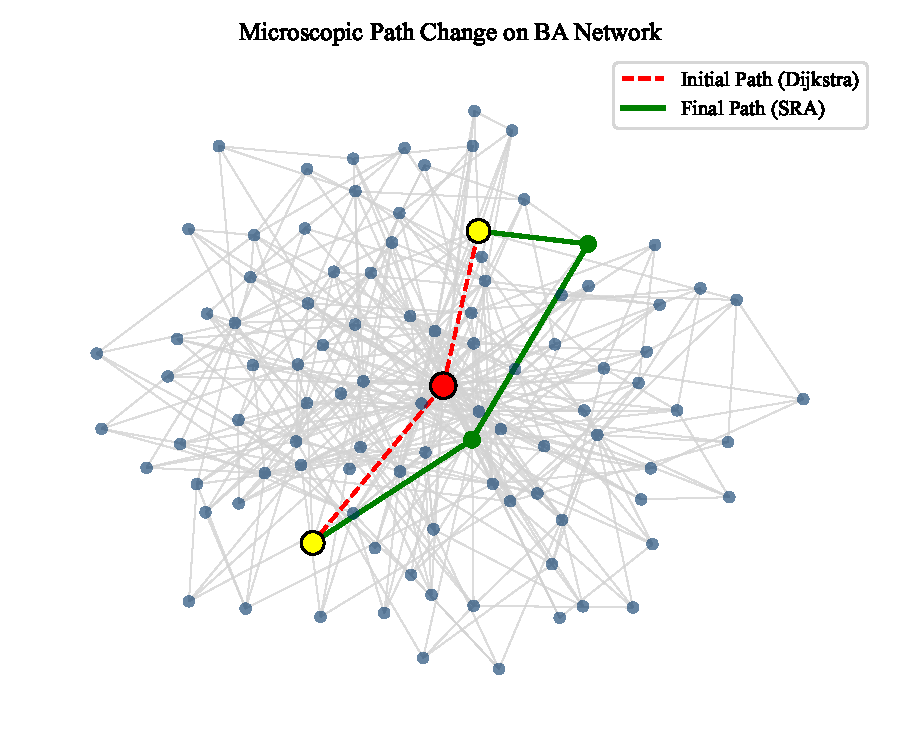
\includegraphics[width=0.8\columnwidth]{figure_7_microscopic_path_change.pdf}
    \caption{SRA 路径重塑机制的概念示意图。算法将业务从穿越中心枢纽、效率高但拥塞严重的 2 跳路径（红色虚线）引导到更长但更加稳定的 4 跳外围路径（绿色实线）。}
    \label{fig:sra_mechanism_visualization}
\end{figure}

\subsection*{复杂度与可扩展性分析}

基线版本的 SRA 每次迭代的计算复杂度由精确中心性计算所主导，利用 Brandes 算法时其复杂度为 $O(N(E + N \log N))$。
在集中式 SDN 部署中，由于控制平面计算与数据平面转发相分离，这一开销是可以接受的。
同时，SRA 还支持一种面向超大规模网络的\textbf{分布式感知模式}。
在这种模式下，我们不再要求精确的全局计算，而是让各个节点作为分布式估计器：它们通过跟踪过境流中不同源宿对的基数，来近似估计自身局部中心性。
随后，这些局部应力指标可通过标准网络管理协议（例如 OSPF-TE 扩展或 SDN 的带内网络遥测）进行高效汇聚，从而将每个节点上的计算复杂度有效降低到 $O(1)$。
这种混合式体系结构保证了 SRA 具备良好的可扩展性与可部署性：在中小规模网络中可采用精确结构分析，而在超大规模环境中则可平滑过渡到统计近似模式。

\subsection{模型收敛性的理论分析}
\label{sec:convergence_analysis}

下面我们为 SRA 控制闭环建立严格的数学基础。
其核心分析难点在于系统的混合特性：一方面，压力状态 $S$ 按连续式规则演化；另一方面，路由拓扑又会发生离散且不连续的切换。
这种非光滑性使得标准基于梯度的控制理论不再适用，也正是启发式协议无法给出稳定性保证的理论障碍所在。

为克服这一问题，我们采用离散时间微分包含系统的形式化工具来建模整个系统动力学。
我们的分析分三步推进，以构造完整的稳定性证明链条：
\begin{enumerate}
    \item \textbf{全局吸引性（安全性）：} 首先证明全局吸引子的存在，保证系统轨迹始终被限制在一个有界安全区域内，不会发散。
    \item \textbf{Lyapunov 衰减（能量性）：} 构造一种专门的\textit{分段 Lyapunov 函数}来量化系统“结构能量”，并证明反馈回路按严格收缩映射持续耗散结构应力。
    \item \textbf{实用稳定性（工程性）：} 最后，我们将最小驻留时间 $T_d$ 形式化为消除高频抖振（Zeno 行为）的必要条件，而非一个经验参数，并据此推导系统收敛到稳定 $\varepsilon$ 邻域的显式速率。
\end{enumerate}

\subsection{全局吸引性与收敛存在性保证}
\label{subsec:attractivity}

基于中心性的路由系统，其收敛性分析之所以困难，根源在于映射 $\kappa(S)$ 具有分段常值、非光滑的特征。
很多启发式方法忽略了路径切换引起的不连续性，因此在理论上留下了空白。
为了建立严格保证，我们并不是对系统进行粗糙近似，而是将这种混合动力学\textbf{正则化}为一个\textbf{离散时间微分包含系统}。
其更新规则被形式化为如下集合值映射：
\begin{equation}\label{eq:inclusion_map}
S^{(k+1)} \in F(S^{(k)}) := (1-\alpha)S^{(k)}+\alpha\,\mathcal{N}(S^{(k)})
\end{equation}
其中，$\mathcal{N}(S)$ 是不连续映射 $\mathrm{norm}(\kappa(\cdot))$ 的\textbf{Krasovskii 正则化}。
从几何意义上讲，该操作在 $S$ 的一个收缩邻域中取所有极限点的凸包，从而有效“填补”由离散路由决策（如并列路径裁决）引起的间隙。
这样便得到一个数学性质良好的映射，并由此导出以下基础性质。

\begin{lemma}[全局约束与安全性]
\label{lemma:invariance}
设状态空间为单位超立方体 $X=[0,1]^N$。
则由 $S^{(k+1)}\in F(S^{(k)})$ 给出的 SRA 离散时间包含系统始终严格受限于 $X$ 内。
形式化地说，$X$ 是一个\textbf{紧致、正不变集合}，并且是一个紧吸收集。
\textit{物理解释：} 该引理保证结构应力不会发散到无穷大；系统具有由归一化机制内生决定的“安全边界”。
\end{lemma}
\begin{IEEEproof}[证明思路]
证明的关键在于：若某一步状态 $S^{(k)}$ 位于超立方体 $X$ 中，则其后继状态 $S^{(k+1)}$ 作为 $X$ 中元素的凸组合，也必然仍位于 $X$ 内。该几何性质直接给出了正不变性。\textit{完整严格证明见附录~\ref{app:proof_lemma_invariance}。}
\end{IEEEproof}

在安全性得到保证之后，我们继续验证控制映射的拓扑正则性。

\begin{proposition}[拓扑正则性]
\label{prop:usc}
由式~\eqref{eq:inclusion_map} 定义的集合值映射 $F(\cdot)$ 是\textbf{上半连续（Upper Semi-Continuous, USC）}的，并且其取值\textbf{非空、紧致且凸}。
\end{proposition}
\begin{IEEEproof}[证明思路]
证明利用了 $\mathcal{N}(S)$ 的分段常值结构，而这一结构来自网络路径配置有限这一事实（见第~\ref{sec:model} 节 A 小节）。该结构保证映射的图是闭的，而在有界空间中，图闭性是 USC 成立的充分条件。\textit{完整严格证明见附录~\ref{app:proof_prop_usc}。}
\end{IEEEproof}

将全局约束性（引理~\ref{lemma:invariance}）与拓扑正则性（命题~\ref{prop:usc}）结合起来，我们便可以刻画系统的最终归宿。

\begin{theorem}[向平衡态的普适收敛]
\label{thm:attractor}
对于离散时间包含系统 \eqref{eq:inclusion_map}，存在一个非空、紧致且正不变的集合 $\Omega\subset X:=[0,1]^N$，称为\textbf{全局吸引子（Global Attractor）}，使得对任意初始状态 $S^{(0)}\in X$，均有：
\begin{equation}\label{eq:attractor_convergence}
\mathrm{dist}\big(S^{(k)},\Omega\big)\ \to\ 0\qquad (k\to\infty).
\end{equation}
\end{theorem}
\begin{IEEEproof}[证明思路]
证明依赖于紧致度量空间上动力系统理论。由于轨迹是预紧的（由引理~\ref{lemma:invariance} 保证），且系统由一个 USC 映射所驱动（命题~\ref{prop:usc}），其 $\omega$-极限集必非空且拟不变。所有此类极限集的并集构成全局吸引子 $\Omega$。\textit{完整严格证明见附录~\ref{app:proof_thm_attractor}。}
\end{IEEEproof}

定理~\ref{thm:attractor} 给出了决定性的结论：SRA 不会出现无界发散。
网络状态将被数学上强制地驱动到一个稳定有界区域 $\Omega$ 中——这正是“弛豫状态”的理论化刻画。

\subsection{能量耗散与有界振荡分析}
\label{subsec:lyapunov}

虽然全局吸引子的存在保证了系统安全，但它并不能定量排除持续振荡（抖振）的可能性。
为了严格表征系统在稳态附近的动力学行为，我们引入非光滑力学中的一个专门分析工具：\textbf{分段 Lyapunov 函数}。
我们构造一个标量函数 $V(S)$ 来量化系统的“结构势能”——定义为当前状态到该瞬时拓扑理想平衡集之间的欧氏距离平方。
形式化地：
\begin{equation}\label{eq:lyapunov_def}
V(S):=\min_{c\in\mathcal N(S)}\|S-c\|_2^2.
\end{equation}
由于 $\mathcal N(S)$ 是紧集，上述最小值是良定义的。
记有限中心性向量集合的最大直径为
$\bar{\Delta} := \max_{i,j} \|v_i - v_j\|$，
它表示最坏情况下的拓扑冲击幅度。
下面的定理揭示了 SRA 控制闭环的基本“热力学”规律。

\begin{theorem}[耗散--注入规律]
\label{thm:drop_jump}
对任意迭代步 $k$，结构能量 $V(S)$ 的演化满足如下“下降--跳变”不等式：
\begin{equation}\label{eq:drop_jump_one_step}
V(S^{(k+1)})\ \le\ \underbrace{(1-\alpha)\,V(S^{(k)})}_{\text{耗散（Drop）}}\ +\ \underbrace{\dfrac{1}{\alpha}\,\bar\Delta^{2}}_{\text{注入（Jump）}}.
\end{equation}
因此，系统能量最终是有界的，并满足如下上极限约束：
\begin{equation}\label{eq:limsup_boundedness}
\limsup_{k\to\infty}V(S^{(k)})\ \le\ \frac{\bar\Delta^{2}}{\alpha^2}.
\end{equation}
\end{theorem}
\begin{IEEEproof}[证明思路]
证明的关键在于对 $V(S)$ 的单步演化进行上界估计。利用加权 Young 不等式，可以将动力学分解为两部分：一部分是由泄漏积分器继承而来的收缩项，另一部分则来自平衡集 $\mathcal N(S)$ 位置变化所带来的有界扰动项。\textit{完整严格证明见附录~\ref{app:proof_thm_drop_jump}。}
\end{IEEEproof}

该定理给出了深刻的物理洞见：SRA 的稳定性由两种相互竞争的机制共同决定。
\textbf{耗散项}（Drop）代表泄漏积分器的阻尼作用，它以 $(1-\alpha)$ 的收缩因子持续从系统中抽取能量；
\textbf{注入项}（Jump）则代表离散拓扑切换给系统带来的能量注入。
由于注入量被 $\bar{\Delta}^2$ 所上界，因此系统最终会进入一个低能轨道，而不是发散失稳。

为了进一步说明采用泄漏积分器的必要性，我们考虑拓扑已经稳定下来的理想情形。

\begin{corollary}[理想条件下的线性收敛]
\label{cor:local_convergence}
当最短路径集合保持不变（即不存在路径切换）时，注入项消失，更新规律退化为一个线性收缩映射：
\begin{equation}\label{eq:linear_update}
S^{(k+1)}=(1-\alpha)S^{(k)}+\alpha c,
\end{equation}
其将以 $(1-\alpha)$ 的速率指数收敛到唯一不动点 $S^\star=c$。
\end{corollary}
\begin{IEEEproof}[证明思路]
证明可直接由 Banach 不动点定理得到。将不动点从更新式中消去后，可得误差动力学
$\|S^{(k+1)}-S^\star\|_2 = (1-\alpha)\|S^{(k)}-S^\star\|_2$，
从而确认其具有完美的指数衰减特性。\textit{完整严格证明见附录~\ref{app:proof_cor_local_convergence}。}
\end{IEEEproof}

\subsection{通过时间正则化获得收敛速率与实用稳定性}
\label{subsec:practical_stability_rate}

“耗散--注入”规律（定理~\ref{thm:drop_jump}）保证了系统能量最终有界。
然而，要从数学上的“有界”真正走向工程上的“可用”，还必须回答两个关键问题：系统究竟以\textit{多快的速度}弛豫到平衡附近？以及我们是否能够严格排除高频\textit{抖振}（Zeno 行为）？
为此，我们引入\textbf{最小驻留时间 $T_d$}，它不是一个经验性补丁，而是混合动力系统所必需的\textbf{时间正则化机制}。
通过将系统演化分解为不同的“驻留块”，我们可以导出显式收敛速率及可调的稳定性保证。

定义第 $m$ 个驻留块为区间 $[\tau_m, \tau_{m+1}-1]$，其中 $\tau_{m+1} = \tau_m + T_d$。
记 $S_m$ 和 $V_m$ 分别为第 $m$ 个驻留块起始时刻的状态与能量。

\begin{proposition}[块级耗散动力学]
\label{prop:block_dynamics}
在时间正则化 $T_d$ 下，拓扑在每个驻留块内部保持不变。
记 $\gamma:=1-\alpha$ 为阻尼因子，$\tilde C:=\bar\Delta^2/\alpha$ 为注入上界，则系统表现出一种\textbf{“先收缩、后跳变”}的行为：
\begin{itemize}
    \item[\textit{(i)}] \textbf{块内冷却：} 在一个驻留块内部，注入项消失，能量呈指数衰减：
    \begin{equation}\label{eq:intra_block}
    V(S^{(\tau_m+t)})\ \le\ \gamma^{\,t}V_m, \quad \text{for } t \in [0, T_d-1].
    \end{equation}
    \item[\textit{(ii)}] \textbf{块间递推：} 相邻驻留块之间的能量状态满足如下线性递推关系：
    \begin{equation}\label{eq:inter_block}
    V_{m+1}\ \le\ \gamma^{T_d}\,V_m\ +\ \tilde C.
    \end{equation}
\end{itemize}
\end{proposition}
\begin{IEEEproof}[证明思路]
(i) 在驻留阶段内，系统退化为纯粹的泄漏积分器（推论~\ref{cor:local_convergence}），因此能量严格按指数规律衰减。
(ii) 上述递推式由两部分组成：前 $T_d-1$ 步的冷却，以及在块边界处发生的一次最坏情况能量注入。\textit{完整严格证明见附录~\ref{app:proof_prop_block_dynamics}。}
\end{IEEEproof}

这一递推关系使我们能够精确计算系统最终静止状态的几何边界。

\begin{theorem}[收敛到可调 $\varepsilon$-吸引域]
\label{thm:epsilon_tube}
设 $\gamma \in (0,1)$ 且 $\tilde C > 0$。
则系统轨迹满足如下严格约束：
\begin{itemize}
    \item[\textit{(a)}] \textbf{稳态半径：} 系统能量最终收敛进入一个有界管状邻域，其半径满足：
    \begin{equation}\label{eq:limsup_radius}
    \limsup_{m\to\infty}V_m\ \le\ \frac{\tilde C}{1-\gamma^{T_d}}.
    \end{equation}
    \item[\textit{(b)}] \textbf{有限时间进入：} 对任意大于上述稳态极限的目标半径 $\varepsilon^2$，系统会在有限步内进入该 $\varepsilon$ 管状邻域，且进入时间可由相应几何级数和的解显式上界。
\end{itemize}
\end{theorem}
\begin{IEEEproof}[证明思路]
对命题~\ref{prop:block_dynamics} 中的递推关系进行迭代展开，即可得到 $V_m$ 被一个收敛几何级数上界所控制，从而收敛到所给出的极限值。\textit{完整严格证明见附录~\ref{app:proof_thm_epsilon_tube}。}
\end{IEEEproof}

最后，我们将上述结果整合为一个明确的工程稳定性保证。

\begin{theorem}[实用稳定性保证]
\label{thm:practical_stability}
当最小驻留时间满足 $T_d \ge 1$ 时，SRA 框架保证：
\begin{itemize}
    \item[\textit{(a)}] \textbf{排除 Zeno 现象：} 切换频率被严格约束在 $1/T_d$ 以内，从而消除了无穷快抖振的风险。
    \item[\textit{(b)}] \textbf{精度可调：} 系统最终误差可以通过调节 $T_d$ 来控制。
\end{itemize}
\end{theorem}
\begin{IEEEproof}[证明思路]
该结论可直接由驻留时间定义与定理~\ref{thm:epsilon_tube} 推出。\textit{完整严格证明见附录~\ref{app:proof_thm_practical_stability}。}
\end{IEEEproof}

式~\eqref{eq:limsup_radius} 还给出了一个闭式设计准则。
给定目标稳定裕量 $R_{\text{target}}^2$，所需的最小驻留时间满足：
\begin{equation}\label{eq:design_parameter_Td}
T_d\ \ge\ \Big\lceil \frac{\ln(1-\tilde C/R_{\text{target}}^2)}{\ln \gamma}\Big\rceil.
\end{equation}
这建立了一个清晰的定量权衡：网络运营者可以通过线性增加稳定化时域 $T_d$，来换取残余能量半径的指数级下降。

\subsection{从结构稳定到容量扩展}
\label{subsec:theory_bridge}

证明系统收敛，意味着系统是安全的；但仅有严格稳定性还不足以说明其工程价值。
我们还必须进一步严格建立\textit{动力学稳定性}与\textit{网络容量}之间的桥梁。
本节将证明：SRA 所达到的平衡集 $\Omega$ 并非任意稳态，而是一个经过结构优化的稳态。
更具体地说，我们将推导出一个形式化联系，说明算法的削峰行为如何直接转化为网络鲁棒容量区域的扩张。

我们首先说明，SRA 控制律会主动抑制“结构奇点”。

\begin{lemma}[削峰机制]
\label{lem:block-budget}
考虑一个包含路径切换事件的驻留时间块 $[\tau_m, \tau_{m+1}]$。
若网络拓扑允许存在备选路径（即不存在严格绑定该业务流的割点），则 SRA 控制律能够保证未归一化峰值中心性严格下降。
形式化地，存在某个 $\delta > 0$，使得：
\begin{equation}
\kappa^{(m+1)}_{\max}\ \le\ \kappa^{(m)}_{\max} - \delta.
\end{equation}
\end{lemma}
\begin{IEEEproof}[证明思路]
这是泄漏积分器逻辑的确定性结果。具有最大中心性的节点会以最快速度积累压力 $S_{\max}$。根据式~\eqref{eq:cost_update}，其节点代价上升得最为剧烈，从而在数学上迫使最短路径算法把业务流转移到低应力的外围节点上，进而降低峰值。\textit{完整严格证明见附录~\ref{app:proof_lem_block_budget}。}
\end{IEEEproof}

这种结构优化——亦即降低负载矩阵的谱半径——会直接映射为性能增益。
为此，我们定义\textit{鲁棒容量下界} $L(\kappa)$。

\begin{proposition}[鲁棒容量区域的扩展]
\label{prop:perf-bridge}
设网络的最小节点服务率为 $\mu_{\min}$。
定义鲁棒容量极限为 $L(\kappa):=\mu_{\min}/\kappa_{\max}$。
记 $\kappa$ 和 $\kappa'$ 分别为 SRA 收敛前后的中心性分布。
由引理~\ref{lem:block-budget} 得到峰值下降 $\kappa'_{\max} < \kappa_{\max}$，则有：
\begin{enumerate}[(i)]
\item \emph{容量严格扩展。} 网络吞吐能力的鲁棒下界严格增加：$L(\kappa') > L(\kappa)$。
\item \emph{瓶颈缓解。} 若网络关键瓶颈恰与拓扑峰值位置对齐（这在无标度网络中是常见情形），则系统实际最大稳定吞吐量 $\rho_{\max}$ 将严格上升。
\end{enumerate}
\end{proposition}
\begin{IEEEproof}[证明思路]
(i) 该结论直接来自容量与瓶颈负载之间的反比关系：当 $\mu_{\min}$ 不变而分母 $\kappa_{\max}$ 降低时，容量区域将单调扩张。
(ii) 由于峰值节点上的绑定约束被缓解，系统得以释放此前无法利用的容量资源。\textit{完整严格证明见附录~\ref{app:proof_prop_perf_bridge}。}
\end{IEEEproof}

\begin{remark}[结构性约束与人为性约束]
必须严格区分由不良路由所造成的\textit{人为拥塞}，与由物理桥接链路或割集所决定的\textit{拓扑硬约束}。
SRA 保证能够消除所有人为性的负载尖峰。
而在存在拓扑硬约束时，尽管系统终极容量仍受物理割集所限制，SRA 仍能够将\textit{有效容量}最大化推进到这一理论极限附近，从而保证网络工作在其 Pareto 最优前沿上。
\end{remark}

\section{仿真分析}
\label{sec:simulation}

第~\ref{sec:model} 节中的理论分析表明，SRA 并不仅仅是一种启发式方法，而是一个受\textit{“耗散--注入规律”}支配的严格控制系统。
本节从数学保证转向经验验证，在随机业务条件下对 SRA 框架进行一次全面的“压力测试”。
我们的实验设计围绕该范式的三个不同层面展开验证：
\begin{enumerate}
    \item \textbf{微观验证（桥梁）：} 首先孤立其核心机制，从经验上验证命题~\ref{prop:perf-bridge}，确认“结构削峰”与“鲁棒容量扩展”之间的确定性联系。
    \item \textbf{宏观涌现（行为）：} 其次分析系统的整体动力学，以揭示其\textit{拓扑依赖型智能}，说明 SRA 如何在异质网络中自主地将目标偏向“性能优化”，而在同质网络中转向“韧性增强”。
    \item \textbf{对比优势（结果）：} 最后，我们将 SRA 与静态协议（Dijkstra）和自适应协议（Q-Routing）进行基准对比，验证其在吞吐扩展性、优雅退化和抗攻击鲁棒性方面的优势。
\end{enumerate}

\subsection{实验设计与环境配置}
\label{subsec:sim_setup}

为了确保实验结果既可复现又具有理论意义，我们构建了一个离散事件仿真环境，用以让各类控制协议承受不同强度的结构应力。
为了严格评估 SRA 的普适性，我们在三类经典网络模型上进行测试，它们覆盖了从高度异质到高度同质的完整拓扑谱系：
\begin{itemize}
    \item \textbf{Barabási-Albert（BA）：} 表示\textit{高度异质}的无标度网络（例如互联网），其特征是幂律度分布以及严重的结构瓶颈。
    \item \textbf{Watts-Strogatz（WS）：} 表示\textit{混合型}小世界网络，兼具较高局部聚类和较短平均路径长度。
    \item \textbf{Erd\H{o}s-Rényi（ER）：} 表示\textit{同质}随机图，作为应力分布相对均匀的对照组。
\end{itemize}

关键仿真参数列于表~\ref{tab:sim_params}。
为了建立有说服力的对比优势，我们选取第~\ref{sec:related_work} 节中三类范式的代表性方法作为基线：
\textbf{Dijkstra}（静态 / 开环）、\textbf{LIRP-D}（反应式 / 对症式）以及 \textbf{Q-Routing}（学习式 / 黑盒）。
其中，Q-Routing 采用标准参数配置（$\alpha=0.1, \gamma=0.9, \epsilon=0.3$），以保证其具有公平的学习能力。
所有结果均报告为\textbf{100 次独立试验}的集合均值，各误差带表示 $\pm1$ 标准差，以保证统计显著性。

\begin{table}[t!]
\centering
\caption{仿真参数汇总。注：``节点服务率''（$\mu_i$）表示控制平面可获得的有效稳态处理预算。}
\label{tab:sim_params}
\renewcommand{\arraystretch}{1.2}
\small
\begin{tabularx}{\columnwidth}{|l|X|}
\hline
\textbf{参数} & \textbf{取值 / 说明} \\
\hline
\hline
\multicolumn{2}{|c|}{\textbf{A. 拓扑谱系（应力条件）}} \\
\hline
网络模型 & BA（异质）、WS（混合）、ER（同质） \\
\hline
默认规模（$N$） & 100 个节点 \\
\hline
BA 连接数（$m$） & 4（高中心性偏斜） \\
\hline
WS 邻居数（$k$） & 8 \\
\hline
WS 重连概率（$p$） & 0.1 \\
\hline
ER 连边概率（$p$） & 0.1 \\
\hline
\hline
\multicolumn{2}{|c|}{\textbf{B. SRA 控制器参数}} \\
\hline
学习率（$\alpha$） & 0.1（记忆保持程度） \\
\hline
积分增益（$\beta_I$） & 10.0（压力-代价敏感度） \\
\hline
最大迭代次数（$K_{\max}$） & 200 \\
\hline
收敛阈值（$\varepsilon$） & $1 \times 10^{-5}$ \\
\hline
\hline
\multicolumn{2}{|c|}{\textbf{C. 业务压力测试参数}} \\
\hline
节点服务率（$\mu$） & 1.0 packet/timestep \\
\hline
总时步数（$T$） & 2000 \\
\hline
预热阶段 & 300 个时步 \\
\hline
节点处理能力 & 10 packets/timestep \\
\hline
节点队列容量 & 50 packets \\
\hline
\end{tabularx}
\end{table}

\subsection{微观验证：机制层面的确认}
\label{subsec:empirical_validation}

在分析宏观业务性能之前，我们首先验证第~\ref{sec:model} 节中推导出的基本机理规律。
更具体地说，我们将算法的核心逻辑单独抽离出来，以验证两个理论命题：其一是“削峰”与“容量扩展”之间的因果联系（命题~\ref{prop:perf-bridge}），其二是“耗散--注入”稳定性动力学（定理~\ref{thm:drop_jump}）。

\begin{figure}[h!]
    \centering
    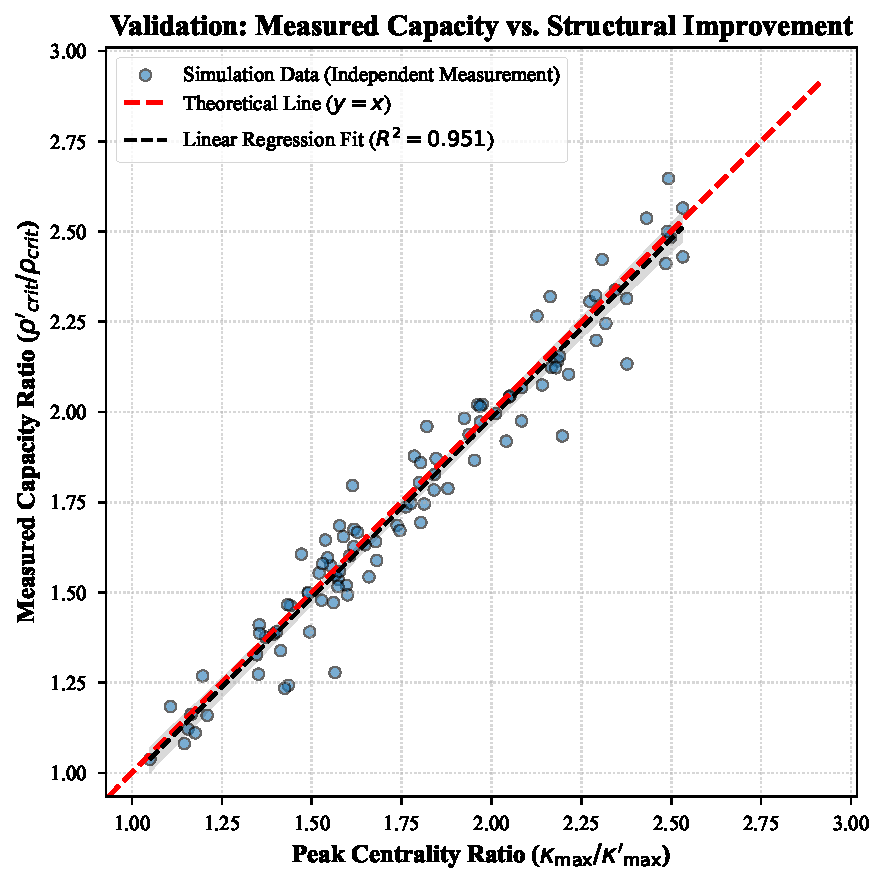
\includegraphics[width=\columnwidth]{ren_fig1_validation.pdf}
    \caption{独立测得的网络容量增益与结构优化比之间的关系。经验数据点紧密聚集在理论预测的 $y=x$ 直线附近，表明性能增益由结构应力分散所确定性驱动。（$R^2=0.951$，样本数 $N=100$）。}
    \label{fig:peak_validation}
\end{figure}

\subsubsection{结构--容量桥梁的验证}

为了验证命题~\ref{prop:perf-bridge} 所预测的确定性联系，我们在 100 个随机网络实例上开展了受控实验。
对于每个实例，我们分别测得两类指标，并据此构成图~\ref{fig:peak_validation} 中的横纵坐标：
\begin{enumerate}
    \item \textbf{理论预测量（X 轴）：} 我们计算\textit{结构优化比}（Structural Optimization Ratio），即 $\kappa_{\max}/\kappa'_{\max}$，它完全依赖于静态图分析。
    \item \textbf{经验真实值（Y 轴）：} 我们通过分组级动态仿真测量\textit{实际容量增益}（Actual Capacity Gain），即 $\rho'_{\text{crit}}/\rho_{\text{crit}}$，该指标独立于中心性计算过程。
\end{enumerate}

如图~\ref{fig:peak_validation} 所示，数据点在 $y=x$ 直线附近呈现高度聚集（$\mathbf{R^2=0.951}$），表明理论预测量能够准确刻画实际物理行为。
这验证了本文的核心主张：性能提升并非偶然现象，而是由结构应力分散所\textbf{确定性驱动}的结果。

\subsection{宏观结构弛豫与平衡态分析}
\label{subsec:dynamic_relaxation}

\begin{table}[h!]
\centering
\caption{SRA 结构优化收益分析（100 次运行的均值 $\pm$ 标准差）}
\label{tab:structural_benefits_stats}
\resizebox{\columnwidth}{!}{
\renewcommand{\arraystretch}{1.2}
\begin{tabular}{|l|l|r|r|r|}
\hline
\textbf{网络} & \textbf{指标} & \textbf{初始值（Dijkstra）} & \textbf{最终值（SRA）} & \textbf{变化（\%）} \\
\hline\hline
ER & 峰值中心性 & $589.93 (\pm 120.59)$ & $209.40 (\pm 26.87)$ & -64.50\% \\
 & 中心性标准差 & $106.93 (\pm 10.62)$ & $33.55 (\pm 9.26)$ & -68.62\% \\
 & 平均路径长度 & $2.25 (\pm 0.04)$ & $2.25 (\pm 0.04)$ & +0.00\% \\
\hline
BA & 峰值中心性 & $2657.37 (\pm 619.87)$ & $431.52 (\pm 45.86)$ & -83.76\% \\
 & 中心性标准差 & $370.10 (\pm 43.87)$ & $91.12 (\pm 6.86)$ & -75.38\% \\
 & 平均路径长度 & $2.37 (\pm 0.02)$ & $2.51 (\pm 0.01)$ & +5.63\% \\
\hline
WS & 峰值中心性 & $856.61 (\pm 169.69)$ & $439.76 (\pm 60.07)$ & -48.66\% \\
 & 中心性标准差 & $175.10 (\pm 22.43)$ & $86.94 (\pm 14.21)$ & -50.35\% \\
 & 平均路径长度 & $3.05 (\pm 0.09)$ & $3.10 (\pm 0.10)$ & +1.78\% \\
\hline
\end{tabular}
}
\end{table}

在完成微观机制验证之后，我们进一步考察 SRA 所达到平衡态的宏观结构属性。
为了保证统计稳健性，我们对每一类拓扑都分析了 100 个独立实例的平均结果。
表~\ref{tab:structural_benefits_stats} 汇总的结果，为 SRA 在不同环境中重塑结构地形的能力提供了定量证据。

数据表明，SRA 具有一种内生的\textit{拓扑依赖型自适应逻辑}。
这种干预在异质的 BA 网络中最为显著，因为这类网络由于其幂律度分布，天然更容易出现“应力奇点”。
在这类环境中，SRA 将峰值中心性降低了 \textbf{83.76\%}，同时将中心性标准差降低了 \textbf{75.38\%}。
更重要的是，这种结构均衡化，也就是“应力分散”仅以相对温和的效率代价实现，平均路径长度只增加了 \textbf{5.63\%}。
这说明 SRA 能够有效识别关键枢纽上的过载压力，并将业务重新分配到此前利用不足的外围路径上。

相比之下，SRA 在更同质的 WS 和 ER 网络中的行为更为保守。
尽管它仍然带来了显著的结构改进，例如，ER 和 WS 网络的峰值中心性分别下降了 64.50\% 和 48.66\%。但对路径效率的影响却几乎可以忽略：WS 的代价低于 2\%，ER 基本为零。
这些结果表明，当底层拓扑本身已经较为均衡时，SRA 不会施加不必要的绕路干预。

总体而言，这些结果支持如下结论：SRA 是一种能够实施“精准治理”的智能控制系统。
它会优先在脆弱拓扑中强化应力再分配，而在稳健拓扑中尽量保持效率，从而在结构稳定性与路由性能之间实现一种拓扑感知的有利平衡。

\subsection{动态性能验证：拓扑感知的二元性}
\label{subsec:dynamic_performance}

前面的结构分析已经确认了应力的有效耗散，而本节进一步通过高保真离散事件仿真来评估这种结构重塑对实际运行关键性能指标（KPI）的影响。
如图~\ref{fig:perf_comparison_stacked} 所示，经验结果表明，SRA 展现出一种涌现式的、与拓扑相关的智能性：它能够根据网络结构约束的不同，自主调整控制目标，从而最大化系统效用。

\paragraph{异质区间（BA 网络）：主动性能优化}
在易形成瓶颈的 BA 拓扑中，SRA 表现为一种\textbf{主动性能优化器}。
如图~\ref{fig:perf_comparison_stacked}(a) 所示，当标准确定性协议和学习型协议都在较低负载下提前饱和时，SRA 的吞吐量却能够随输入负载近似线性扩展，在高应力场景下几乎将网络的可运行容量提升到原来的两倍。
这种收益源于 SRA 能够在物理队列溢出之前主动转移业务流，因此即便在基准方法丢包率超过 40\% 并出现灾难性失效的区间内，SRA 仍可将丢包率维持在 10\% 以下。

\paragraph{混合区间（WS 网络）：稳定性保障}
WS 网络的结果（图~\ref{fig:perf_comparison_stacked}(b)）凸显了 SRA 在\textbf{保障系统稳定性}方面的作用。
在低负载时，各种协议的行为基本一致；然而，一旦系统进入“拥塞拐点”（负载 $> 1.0$），它们的表现便迅速分化。
值得注意的是，学习驱动的 Q-Routing 在这一阶段发生了灾难性崩溃，无法适应快速变化的系统状态。
相比之下，SRA 能够平滑地穿越这一高风险区间，即使在极端饱和条件下，仍然保持稳定吞吐和受控丢包，从而实现“优雅退化”。

\paragraph{同质区间（ER 网络）：韧性增强}
在 ER 拓扑中，由于不存在支配性枢纽，可用于扩展吞吐的结构空间本身就十分有限，因此 SRA 会智能地转化为一种\textbf{韧性增强机制}。
虽然各类协议的吞吐量几乎没有差异，但 SRA 始终能够把丢包率压制在约 2\% 左右，相较于其他方法约 7\% 的水平有显著改善。
与此同时，我们也观察到平均时延出现了可预期的上升。
这反映了一种合理且自适应的“以时延换可靠性”权衡：SRA 控制器识别出吞吐扩展已经受到结构性上限约束，因此转而优先保障分组交付的完整性。

\begin{figure*}[t!]
    \centering
    % (a) BA Network Plot
    \begin{subfigure}{\textwidth}
        \centering
        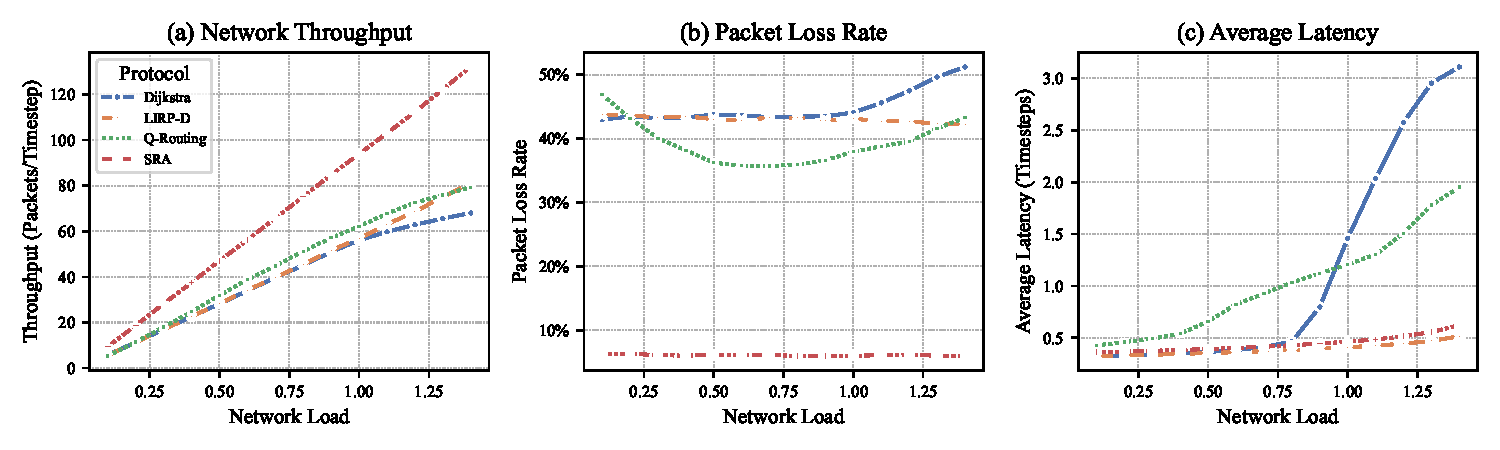
\includegraphics[width=0.95\textwidth]{performance_comparison_ba.pdf}
        \caption{BA 网络上的性能表现。SRA 在这里表现为一个\textbf{主动性能优化器}，有效将吞吐扩展能力与结构瓶颈解耦。}
        \label{fig:perf_ba_stacked}
    \end{subfigure}
    
    \vspace{0.5cm}

    % (b) WS Network Plot
    \begin{subfigure}{\textwidth}
        \centering
        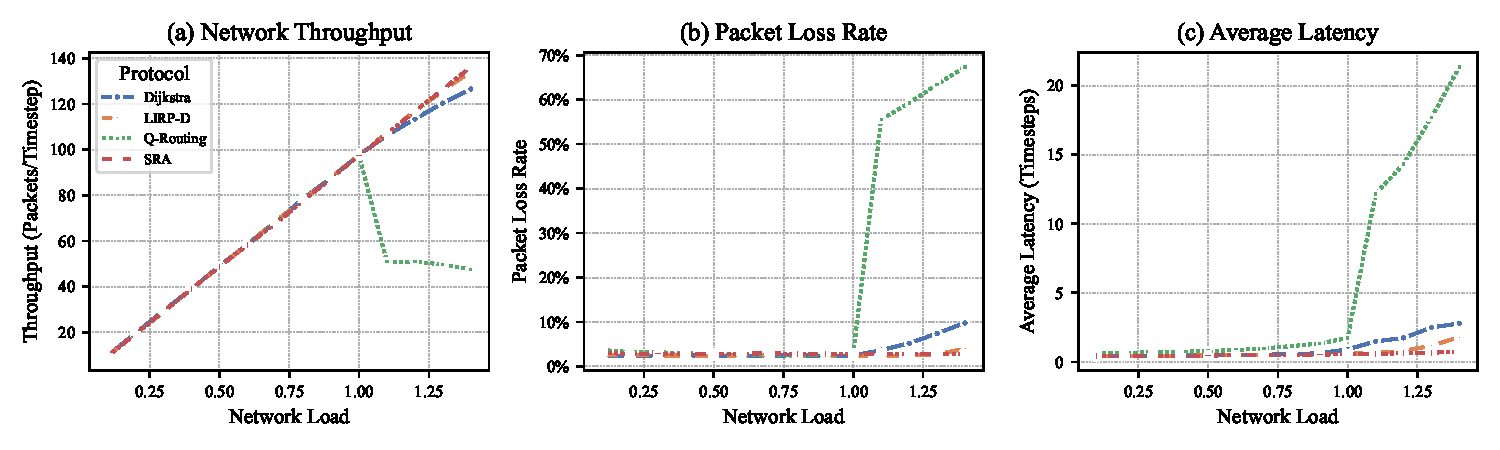
\includegraphics[width=0.95\textwidth]{performance_comparison_ws.pdf}
        \caption{WS 网络上的性能表现。SRA 能够在关键“拥塞拐点”之后继续保持稳定运行，从而避免学习型方法中观察到的灾难性崩溃。}
        \label{fig:perf_ws_stacked}
    \end{subfigure}

    \vspace{0.5cm}

    % (c) ER Network Plot
    \begin{subfigure}{\textwidth}
        \centering
        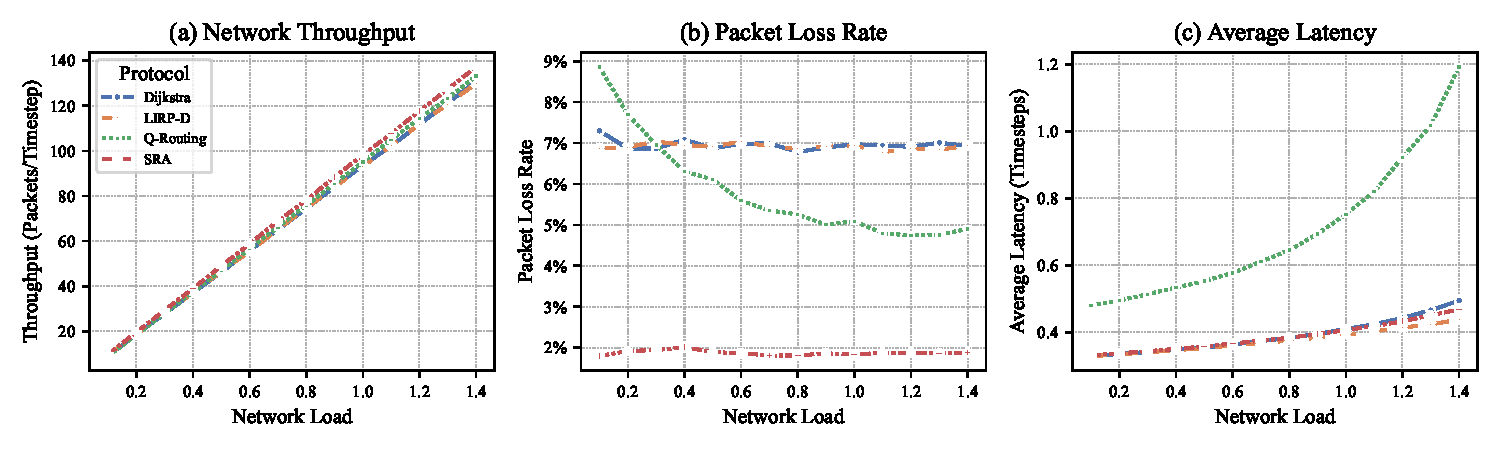
\includegraphics[width=0.95\textwidth]{performance_comparison_er.pdf}
        \caption{ER 网络上的性能表现。在缺乏可利用结构差异的情况下，SRA 表现为一种韧性增强机制，通过自适应权衡来尽可能降低丢包率\cite{Mendonca2021ApproxCentrality}。}
        \label{fig:perf_er_stacked}
    \end{subfigure}
    
    \caption{不同拓扑谱系下的动态业务性能对比。结果表明，SRA 能够根据底层网络结构的不同，自动调整其控制策略\cite{Cheng2010SelfOrganizingModel}。}
    \label{fig:perf_comparison_stacked}
\end{figure*}

\subsection{对抗鲁棒性：面向定向攻击的韧性表现}
\label{subsec:robustness_and_params}

为了评估 SRA 范式在生存性方面的实际价值，我们进一步在网络中引入了\textbf{定向节点移除}的对抗场景。
具体地，节点按其初始介数中心性（BC）从高到低依次移除，这相当于模拟一种最坏情形：攻击者优先破坏拓扑中最关键的枢纽节点。
我们使用相对于基线 Dijkstra 策略的\textbf{SRA PDR 优势}来量化韧性增益：
\begin{equation}
\label{eq:pdr_advantage}
\text{Advantage (\%)} = \frac{\text{PDR}_{\text{SRA}} - \text{PDR}_{\text{Dijkstra}}}{\text{PDR}_{\text{Dijkstra}}} \times 100\%
\end{equation}
结果取自 50 次独立对抗试验的平均值，并绘制于图~\ref{fig:robustness_summary_stats} 中。

结果为 SRA 的\textbf{脆弱性感知智能}提供了有力的统计证据：
\begin{itemize}
    \item \textbf{在异质 BA 网络中：} SRA 在整个攻击过程中都能持续提供超过 60\% 的 PDR 优势。由于它在攻击发生之前就已经主动分散了结构应力，因此单个枢纽节点的失效不会再触发剩余路径的灾难性崩溃。
    \item \textbf{在混合型 WS 网络中：} 这种韧性增益具有明显的\textit{涌现性}。在轻度损伤时优势较小，但当网络遭受较为严重的结构破坏后，其优势可上升到约 20\%，说明 SRA 能够围绕残余拓扑片段动态重组业务流。
    \item \textbf{在同质 ER 网络中：} SRA 基本维持中性（0\%）优势。这一点非常重要：它说明在本身就具有较高路径冗余、天然稳健的拓扑中，SRA 会\textit{正确地避免不必要干预}，从而不会在不存在结构脆弱性的地方额外引入开销。
\end{itemize}

这种行为表明，SRA 是一种精确的治理机制：在真正需要时它会积极介入，而在不需要时则保持克制，从而维持一种轻量但稳健的网络状态。

\begin{figure}[t!]
    \centering
    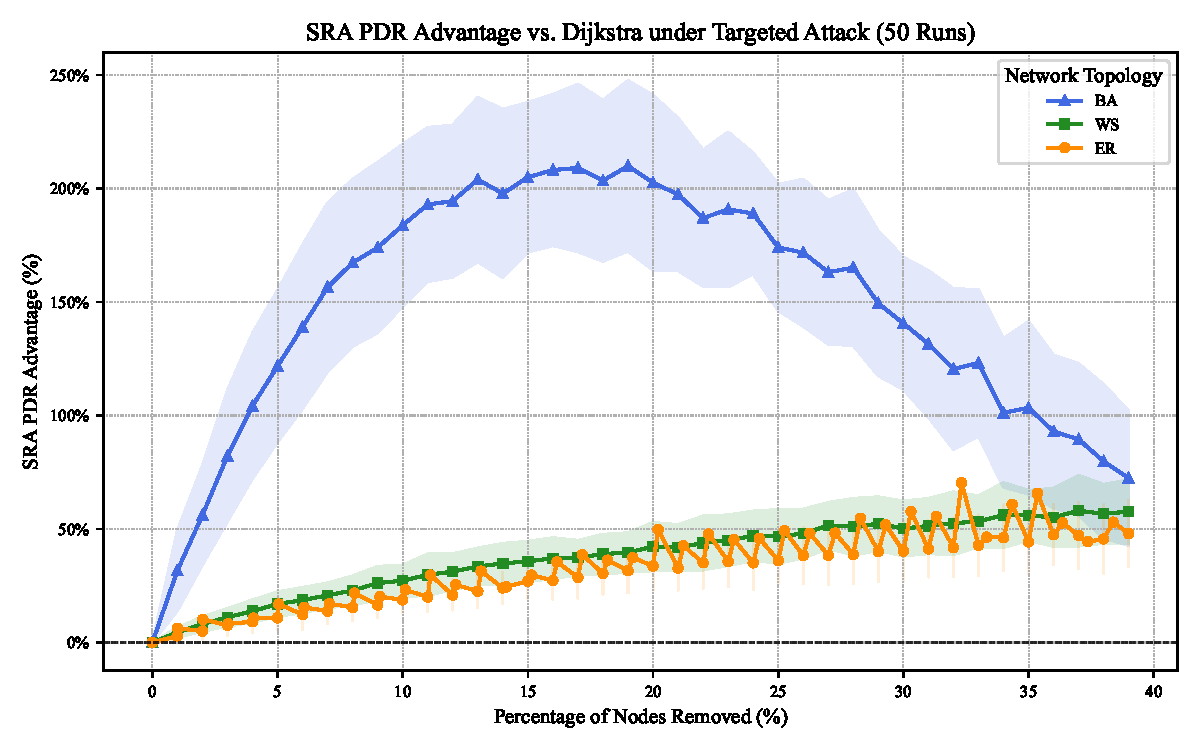
\includegraphics[width=\columnwidth]{robustness_advantage_summary_stats.pdf}
    \caption{定向枢纽移除攻击下，SRA 相对于 Dijkstra 的 PDR 优势\cite{Basaras2019Influential}。结果验证了 SRA 在脆弱网络（BA）中提供拓扑加固能力、并在混合型网络（WS）中提供自适应生存能力的效果。}
    \label{fig:robustness_summary_stats}
\end{figure}

\section{讨论与结论}
\label{sec:discussion_conclusion}

本文提出、分析并验证了系统弛豫算法（System Relaxation Algorithm, SRA），将其作为针对传统网络控制中普遍存在的“应力集中”问题的一种模型驱动型响应机制。
通过综合网络科学与非光滑动力系统的理论思想，我们为 SRA 建立了严格的理论基础，并首次为处理不连续路径切换动力学的这类系统给出了形式化稳定性保证。
大规模经验评估进一步明确表明，SRA 超越了反应式启发方法的局限，展现出一种深刻的、依赖于拓扑结构的智能性。

SRA 的战略价值，在于它能够以智能且具备拓扑感知能力的方式处理\textbf{性能与韧性之间的基本权衡}。
实验结果表明，SRA 可被视为一种自适应治理器，其具体策略由网络底层结构约束所决定：
\begin{itemize}
    \item \textbf{在异质拓扑中：} SRA 充当一种\textit{主动性能优化器}，以较小的效率代价换取容量的大幅扩展，这一点可由峰值中心性降低 80\% 的结果充分说明。
    \item \textbf{在同质拓扑中：} 它的目标则会自动转向\textit{韧性增强}，通过更细粒度的调节，提前管理动态拥塞与结构损伤带来的风险。
\end{itemize}

更为关键的是，SRA 的行为所收敛到的并不是一个脆弱的静态不动点，而是一个\textbf{鲁棒的动态平衡}。
这是系统的一个深层特征，其根源在于路径选择内在的非光滑性。
“泄漏积分器”机制正是为管理这种动力学而设计，它提供了必要的记忆性与阻尼，使系统能够表现出可预测、有界且远比静态最优点更能抵御现实扰动的行为。

若将其放到现代网络体系结构中考察，SRA 可被视为一种十分有力的、面向 SDN 控制器的白盒控制应用，因为 SDN 控制器天然具备进行应力分析所需的全局视图，以及执行集中式策略下发所需的控制权限。
本文为模型驱动型韧性网络建立了理论基石，同时也打开了若干值得继续深入的研究方向，包括：与生产级 SDN 控制器的集成、在真实 ISP 拓扑上的验证，以及自调参机制的设计，以进一步提升其自适应精度。


\bibliographystyle{IEEEtran}
\bibliography{refs}


\appendices
\section{引理 \ref{lemma:invariance} 的证明}
\label{app:proof_lemma_invariance}
\begin{IEEEproof}
\textit{(a) 正不变性：}
任取 $S^{(k)}\in X$。
由最大值归一化可知，$\mathcal N(S^{(k)})\subset[0,1]^N=X$。
对任意选择的 $c^{(k)}\in\mathcal N(S^{(k)})$ 以及任意坐标 $i$，有
\begin{equation}
S^{(k+1)}_i=(1-\alpha)S^{(k)}_i+\alpha\,c^{(k)}_i,
\quad\text{其中}\quad S^{(k)}_i,c^{(k)}_i\in[0,1].
\end{equation}
因此，
\begin{equation}
0\cdot(1-\alpha)+0\cdot\alpha\ \le\ S^{(k+1)}_i\ \le\ 1\cdot(1-\alpha)+1\cdot\alpha,
\end{equation}
从而推出 $S^{(k+1)}_i\in[0,1]$。
由于这对每个坐标都成立，因此有 $S^{(k+1)}\in X$。
这表明 $F(X)\subset X$：\textbf{若当前时刻状态位于 $X$ 中，则下一时刻状态仍位于 $X$ 中}。
因此，$X$ 是一个正不变集合。

\textit{(b) 紧致性：}
集合 $X=[0,1]^N$ 是一个闭且有界的超立方体，因此它是紧集。

\textit{(c) “有效状态空间”上的吸收性：}
本文中的算法与分析都在 $X$ 内初始化（即 $S^{(0)}\in X$），且由 (a) 可知 $F(X)\subset X$。
因此，对于定义在状态空间 $X$ 上的离散时间半流
\begin{equation}
\Phi(k,\cdot):X\to 2^X,\quad \Phi(1,\cdot)=F,\ \ \Phi(k+1,\cdot)=F\circ\Phi(k,\cdot),
\end{equation}
集合 $X$ \textbf{吸收其自身}：对任意有界集合 $B\subset X$，取 $n_B=0$ 即有 $\Phi(n,B)\subset X$ 对所有 $n\ge 0$ 成立。
按照标准定义，这意味着 \textbf{$X$ 是一个紧吸收集}。

由此可得
\begin{equation}
\delta^+_{k+1,i}\ \le\ (1-\alpha)\,\delta^+_{k,i},\qquad 
\delta^-_{k+1,i}\ \le\ (1-\alpha)\,\delta^-_{k,i}.
\end{equation}
这意味着 $\max\{\delta^+_{k,i},\delta^-_{k,i}\}$ 以速率 $1-\alpha$ 几何收敛到 0，因此
$\mathrm{dist}_\infty(S^{(k)},X)\le (1-\alpha)^k\,\mathrm{dist}_\infty(S^{(0)},X)\to0$。
这说明系统对 $X$ 具有\textbf{指数吸引性}。
本文主过程本身就在 $X$ 内初始化，因此 (c) 中的吸收集表述已足够满足需求。

综上，$X=[0,1]^N$ 对该系统而言是正不变且紧致的，同时在以 $X$ 为状态空间的离散时间半流意义下，它也是一个紧吸收集。
\end{IEEEproof}

\section{命题 \ref{prop:usc} 的证明}
\label{app:proof_prop_usc}
\begin{IEEEproof}
\textit{(a) 非空、紧致且凸的取值：}
根据第三章 A 节中的定义，$\mathrm{norm}(\kappa(S))\in[0,1]^N$。
因此，对任意 $S$，有
\begin{equation}
\mathcal N(S)=\mathrm{co}\!\big(\mathrm{norm}(\kappa(S))\big)\subset[0,1]^N.
\end{equation}
非空集合的闭凸包 $\mathrm{co}(\cdot)$ 仍然是\textbf{非空}的。
同时，它还是 $[0,1]^N$ 中一个\textbf{闭且有界}的凸子集，因此它必然是\textbf{紧致}且\textbf{凸}的。

\textit{(b) 分段常值结构与有限性：}
图 $G$ 以及源宿（OD）对集合都是有限的。
节点代价 $C(S)$ 是 $S$ 的仿射函数。
对于每一个 OD 对 $(s,t)$，候选简单路径集合都是\textbf{有限}的。
每条路径的代价，都是关于 $S$ 的一族仿射函数的\textbf{逐点最小值}。
因此，状态空间中存在一个\textbf{有限划分}，使得在每一个划分区域内，所有 OD 对的最短路径集合都保持\textbf{不变}。
由此可知，在每个划分内部，$\kappa(S)$ 与 $\mathrm{norm}(\kappa(S))$ 都是\textbf{常向量}。
在这些划分边界上，$\mathrm{norm}(\kappa(S))$ 的极限只能取自相邻划分对应的\textbf{有限个常向量}。
记这些常向量为 $\{v_\ell\}_{\ell\in\mathcal I(S)}$，其中 $\mathcal I(S)$ 表示与 $S$ 相邻的划分索引的有限集合，则有
\begin{equation}
\mathcal N(S)=\mathrm{co}\big(\{v_\ell:\,\ell\in\mathcal I(S)\}\big).
\end{equation}
这就说明，$\mathcal N(\cdot)$ 具有一种\textbf{分段常值、边界处取闭凸包}的结构。

\textit{(c) 通过序列判据 / 闭图性质证明上半连续（USC）：}
任取一列 $S_n\to S$，并令 $c_n\in\mathcal N(S_n)$ 且 $c_n\to c$。
我们需要证明 $c\in\mathcal N(S)$。
由 (b) 可知，对每个 $n$，存在有限集合 $\{v_{\ell}: \ell\in\mathcal I(S_n)\}$，使得
$c_n\in\mathrm{co}\big(\{v_{\ell}:\ell\in\mathcal I(S_n)\}\big)$。
由 Carathéodory 定理，我们可将其写为
\begin{equation}
c_n=\sum_{j=0}^{N} \lambda_{n,j}\, v_{\ell_{n,j}},\quad 
\lambda_{n,j}\ge 0,\ \sum_{j=0}^{N}\lambda_{n,j}=1,\ 
\ell_{n,j}\in\mathcal I(S_n).
\end{equation}
由于这些向量 $v_{\ell}$ 来自一个\textbf{全局有限}集合 $\{v_1,\dots,v_M\}$，因此我们可以抽取一个子列，使得 $\ell_{n,j}\equiv \bar\ell_j$ \textbf{固定不变}，同时（利用 $[0,1]$ 的紧致性）有 $\lambda_{n,j}\to \bar\lambda_j$。
于是，
\begin{equation}
c=\lim_{n\to\infty} c_n=\sum_{j=0}^{N}\bar\lambda_j\, v_{\bar\ell_j},
\quad\sum_{j=0}^{N}\bar\lambda_j=1,\ \bar\lambda_j\ge 0.
\end{equation}
由于 $S_n\to S$，当 $n$ 足够大时，任一极限索引 $\bar\ell_j$ 都必须属于 $\mathcal I(S)$。
因此，每个极限向量 $v_{\bar\ell_j}$ 都是与 $S$ 相邻划分中的常向量之一。
于是，
\begin{equation}
c=\sum_{j=0}^{N}\bar\lambda_j\, v_{\bar\ell_j}\ \in\ 
\mathrm{co}\big(\{v_\ell:\,\ell\in\mathcal I(S)\}\big)=\mathcal N(S).
\end{equation}
这就说明，$\mathcal N$ 的图
$\mathrm{gph}\,\mathcal N:=\{(S,c):\,c\in\mathcal N(S)\}$
是闭的。
具有紧取值的闭图映射必然是\textbf{上半连续}的。

\textit{(d) $F(\cdot)$ 的性质：}
缩放与平移保持 USC 性以及非空、紧致、凸取值这些性质。
映射 $S\mapsto (1-\alpha)S$ 是连续的（单值映射）。
因此，连续映射与 USC 映射的 Minkowski 和
$F(S)=(1-\alpha)S+\alpha\,\mathcal N(S)$
仍然是 USC 的，并且具有非空、紧致和凸的取值。
\end{IEEEproof}

\section{定理 \ref{thm:attractor} 的证明}
\label{app:proof_thm_attractor}
\begin{IEEEproof}
\textit{(a) 预紧性：}
由引理 \ref{lemma:invariance} 可知，$X=[0,1]^N$ 是一个紧致且正不变的集合。
因此，任意从 $X$ 出发的轨迹都会始终留在 $X$ 中。
由于 $X$ 是紧集，任意轨迹都是\textbf{预紧}的（即存在收敛子列）。

\textit{(b) $\omega$-极限集的存在性：}
对任意 $S^{(0)}\in X$，其 $\omega$-极限集定义为
\begin{equation}
\omega\big(S^{(0)}\big)\ :=\ \left\{x\in X:\ \exists\,k_n\uparrow\infty\ \text{s.t.}\ S^{(k_n)}\to x\right\}.
\end{equation}
由预紧性可知，$\omega(S^{(0)})$ 是\textbf{非空}且\textbf{紧致}的。

\textit{(c) $\omega$-极限集的正不变性：}
由命题 \ref{prop:usc} 可知，$F(\cdot)$ 是 USC 的且具有紧取值，这意味着它的图是闭的。
任取 $x \in \omega(S^{(0)})$。
根据定义，存在子列 $S^{(k_n)} \to x$。
相应的后继点 $S^{(k_n+1)} \in F(S^{(k_n)})$ 位于紧集 $X$ 内，因此还可抽取进一步子列，使其收敛为 $S^{(k_n+1)} \to y$。
由闭图性质可知，$y \in F(x)$。
由于 $\{k_n+1\}$ 同样趋于无穷，因此 $y$ 也属于 $\omega(S^{(0)})$。
故有
\begin{equation}
F\big(\omega(S^{(0)})\big)\ \subset\ \omega(S^{(0)}).
\end{equation}

\textit{(d) 轨迹对 $\omega$-极限集的吸引性：}
可以通过反证法证明，轨迹必然逼近其对应的 $\omega$-极限集。
因此，
\begin{equation}
\mathrm{dist}\big(S^{(k)},\omega(S^{(0)})\big)\ \to\ 0.
\end{equation}

\textit{(e) 全局吸引子：}
令 $\Omega$ 为所有初始点在 $X$ 中的 $\omega$-极限集的并：
\begin{equation}
\Omega\ :=\ \bigcup_{S^{(0)}\in X} \omega(S^{(0)}).
\end{equation}
集合 $\Omega$ 非空、紧致且正不变。
对任意 $S^{(0)}\in X$，由于 $\mathrm{dist}(S^{(k)},\omega(S^{(0)}))\to 0$ 且 $\omega(S^{(0)})\subset\Omega$，因此有
\begin{equation}
\mathrm{dist}\big(S^{(k)},\Omega\big)\ \to\ 0.
\end{equation}
因此，$\Omega$ 是该系统的全局吸引子。
\end{IEEEproof}

\section{定理 \ref{thm:drop_jump} 的证明}
\label{app:proof_thm_drop_jump}
\begin{IEEEproof}
令 $c_k\in\arg\min_{c\in\mathcal N(S^{(k)})}\|S^{(k)}-c\|_2^2$，于是
$V(S^{(k)})=\|S^{(k)}-c_k\|_2^2$。
根据离散时间包含关系，取
\begin{equation}
S^{(k+1)}=(1-\alpha)S^{(k)}+\alpha\,c_k.
\end{equation}
再令 $c_{k+1}\in\mathcal N(S^{(k+1)})$ 为 $V(S^{(k+1)})$ 的一个极小化点。
则可写为
\begin{equation}
S^{(k+1)}-c_{k+1}=(1-\alpha)(S^{(k)}-c_k) + (c_k-c_{k+1}).
\end{equation}
应用加权 Young 不等式
$\|x+y\|_2^2\le (1+\lambda)\|x\|_2^2+(1+1/\lambda)\|y\|_2^2$，
并取 $\lambda=\alpha/(1-\alpha)$，可得
\begin{equation}
\|S^{(k+1)}-c_{k+1}\|_2^2 \le (1-\alpha)\|S^{(k)}-c_k\|_2^2 + \frac{1}{\alpha}\,\|c_k-c_{k+1}\|_2^2.
\end{equation}
由于 $c_k$ 与 $c_{k+1}$ 都属于一个有限向量集的凸包，因此二者之间的距离有界，即
$\|c_k-c_{k+1}\|\le \bar\Delta$。
将其代入即可得到所需不等式。
上极限结果则可由求解相应线性递推不等式直接得到。
\end{IEEEproof}

\section{推论 \ref{cor:local_convergence} 的证明}
\label{app:proof_cor_local_convergence}
\begin{IEEEproof}
(1) \textbf{不动点的唯一性：}
求解
$S=(1-\alpha)S+\alpha c$
可得
$\alpha S=\alpha c$，
因此 $S=c$。
故唯一不动点为 $S^\star=c$。

(2) \textbf{压缩性与收敛速率：}
\begin{equation}
S^{(k+1)}-c = (1-\alpha)S^{(k)}+\alpha c-c = (1-\alpha)\big(S^{(k)}-c\big).
\end{equation}
取 2-范数并迭代，可得
\begin{equation}
\|S^{(k)}-S^\star\|_2 = (1-\alpha)^k\,\|S^{(0)}-S^\star\|_2.
\end{equation}
\end{IEEEproof}

\section{命题 \ref{prop:block_dynamics} 的证明}
\label{app:proof_prop_block_dynamics}
\begin{IEEEproof}
(i) 在一个驻留块内部，$\mathcal N(S)\equiv\{c_m\}$ 为常值。
因此，定理 \ref{thm:drop_jump} 中不等式的“跳变”项为零。
于是有
$V_{k+1}\le \gamma V_k$，
连续迭代 $t$ 次即可得到结论。

(ii) 在第 $m$ 个块与第 $m+1$ 个块的边界处，允许发生一次切换。
对这一步应用定理 \ref{thm:drop_jump} 中的“下降--跳变”不等式：
\begin{equation}
\begin{split}
V_{m+1} = V(S^{(\tau_{m+1})}) & \le \gamma\,V(S^{(\tau_{m+1}-1)}) + \tilde C \\
& = \gamma\,V(S^{(\tau_m+T_d-1)}) + \tilde C \\
& \le \gamma \cdot (\gamma^{T_d-1}V_m) + \tilde C = \gamma^{T_d}V_m + \tilde C,
\end{split}
\end{equation}
其中最后一个不等式使用了 (i) 的结果。
\end{IEEEproof}

\section{定理 \ref{thm:epsilon_tube} 的证明}
\label{app:proof_thm_epsilon_tube}
\begin{IEEEproof}
(a) 对命题 \ref{prop:block_dynamics}(ii) 中的线性递推式
$V_{m+1}\le \gamma^{T_d}V_m+\tilde C$
进行迭代展开，有
\begin{equation}
\begin{split}
V_m &\le (\gamma^{T_d})^m V_0 + \tilde C \sum_{j=0}^{m-1}(\gamma^{T_d})^j \\
    &= \gamma^{mT_d}V_0 + \tilde C\,\frac{1-\gamma^{mT_d}}{1-\gamma^{T_d}} \\
    &\le \gamma^{mT_d}V_0+\frac{\tilde C}{1-\gamma^{T_d}}.
\end{split}
\end{equation}
令 $m\to\infty$ 取上极限，即得到稳态半径结论。

(b) 令 $V_m\le \varepsilon^2$，并利用 (a) 中的上界求解 $m$，即可得到相应结果。
\end{IEEEproof}

\section{定理 \ref{thm:practical_stability} 的证明}
\label{app:proof_thm_practical_stability}
\begin{IEEEproof}
(a) 根据最小驻留时间的定义，一次切换发生后，至少在接下来的 $T_d$ 个时步内不允许再次切换。
因此，在长度为 $T$ 的任意时间窗口中，切换次数都被严格上界。

(b) 该结论可由求解块间递推关系直接得到，如定理 \ref{thm:epsilon_tube}(a) 的证明所示。

(c) 该结果由对定理 \ref{thm:epsilon_tube}(b) 中不等式进行反求可直接得到。
\end{IEEEproof}

% --- START: New Appendices for Section III-E ---

\section{引理~\ref{lem:block-budget} 的证明}
\label{app:proof_lem_block_budget}
\begin{IEEEproof}
该证明由两个部分组成：一是给出非峰值节点增量的上界，二是保证峰值节点的严格下降。

\noindent\textit{1) 非峰值增量上界：}
设 $c^{(m)}$ 与 $c^{(m+1)}$ 分别表示该块起始与结束时的归一化中心性向量。
根据 $\bar\Delta$ 的定义，有
$\|c^{(m+1)}-c^{(m)}\|_\infty \le \bar\Delta$，
即对任意 $j$ 都有
$|c^{(m+1)}_j - c^{(m)}_j| \le \bar\Delta$。
对应的未归一化中心性为
$\kappa^{(m)}_j = c^{(m)}_j \kappa^{(m)}_{\max}$，
以及
$\kappa^{(m+1)}_j = c^{(m+1)}_j \kappa^{(m+1)}_{\max}$。
由于峰值中心性不会上升（事实上会下降，这一点随后将证明），因此有
$\kappa^{(m+1)}_{\max} \le \kappa^{(m)}_{\max}$。
于是，对于任意非峰值节点 $j \neq u$，有

\begin{align*}
\kappa^{(m+1)}_j - \kappa^{(m)}_j &= c^{(m+1)}_j \kappa^{(m+1)}_{\max} - c^{(m)}_j \kappa^{(m)}_{\max} \\
&\le c^{(m+1)}_j \kappa^{(m)}_{\max} - c^{(m)}_j \kappa^{(m)}_{\max} \\
&= (c^{(m+1)}_j - c^{(m)}_j) \kappa^{(m)}_{\max} \\
&\le |c^{(m+1)}_j - c^{(m)}_j| \kappa^{(m)}_{\max} \le \bar\Delta \cdot \kappa^{(m)}_{\max} =: B^{(m)}.
\end{align*}

\noindent\textit{2) 保证峰值下降（$\delta>0$）：}
峰值存在净下降这一事实，直接来源于第~\ref{sec:convergence_analysis} 节所证明的系统动力学性质。
“下降--跳变”不等式（定理~\ref{thm:drop_jump}）以及驻留时间策略（定理~\ref{thm:practical_stability}）共同保证：系统不会停留在一个固定不变点，而会在一个稳定吸引子内持续演化，从而必然触发状态转移。

一次状态转移（即路径切换）发生的条件是：高中心性节点 $u$ 的代价
$C_u = 1 + \beta_I S_u$
增大到足以使替代路径变得更便宜。
状态更新律
$S_u^{(k+1)} = (1-\alpha)S_u^{(k)} + \alpha c_u^{(k)}$
保证：具有峰值归一化中心性（$c_u=1$）的节点，其压力增长速度最快。

这一机制必然保证业务流最终从峰值节点 $u$ 上转移出去。
由于假设网络中不存在结构上不可避免的瓶颈，因此这种转移必然导致其未归一化中心性 $\kappa_u$ 严格下降。
因此，对任意包含此类路径切换事件的驻留块，都必然存在某个净下降量 $\delta > 0$。
$\delta$ 的具体大小依赖于系统参数（$\alpha, \beta_I, T_d$）以及网络拓扑，但它的存在性由收敛动力学严格保证。
\end{IEEEproof}

\section{命题~\ref{prop:perf-bridge} 的证明}
\label{app:proof_prop_perf_bridge}
\begin{IEEEproof}
该证明利用了引理~\ref{lem:block-budget} 所保证的峰值严格下降性质，即
$\kappa'_{\max} < \kappa_{\max}$。

\noindent\textit{(i) 无条件鲁棒下界：}
鲁棒容量下界定义为
$L(\kappa) := \mu_{\min}/\kappa_{\max}$。
由于 SRA 不会改变节点的物理服务率，因此 $\mu_{\min}$ 为常数。
又因为 $\kappa'_{\max} < \kappa_{\max}$，故直接有：
\begin{equation}
L(\kappa') = \frac{\mu_{\min}}{\kappa'_{\max}} > \frac{\mu_{\min}}{\kappa_{\max}} = L(\kappa).
\end{equation}
因此，该容量下界严格上升。

\noindent\textit{(ii) 对齐瓶颈下的容量增益：}
网络容量定义为
\begin{equation}
\rho_{\max}(\kappa) = \min_{i \in V} \frac{\mu_i}{\kappa_i}.
\end{equation}
SRA 作用后的新容量为
\begin{equation}
\rho_{\max}(\kappa') = \min_{i \in V} \frac{\mu_i}{\kappa'_i}.
\end{equation}
根据最小值定义，一个集合的最小值必然不大于其中任意单个元素。
因此，新容量以下式为下界，其中 $u$ 是原始峰值节点：
\begin{equation}
\rho_{\max}(\kappa') \ge \frac{\mu_u}{\kappa'_u}.
\end{equation}
进一步地，由于在新的状态 $\kappa'$ 中，$u$ 未必仍是峰值节点，因此其中心性 $\kappa'_u$ 必然不大于新的峰值中心性 $\kappa'_{\max}$。
于是有：
\begin{equation}
\rho_{\max}(\kappa') \ge \frac{\mu_u}{\kappa'_u} \ge \frac{\mu_u}{\kappa'_{\max}}.
\end{equation}
而本情形的前提是：原始系统的瓶颈恰好位于峰值节点，因此
$\rho_{\max}(\kappa) = \mu_u/\kappa_{\max}$。
将上述关系联立即得：
\begin{equation}
\rho_{\max}(\kappa') \ge \frac{\mu_u}{\kappa'_{\max}} > \frac{\mu_u}{\kappa_{\max}} = \rho_{\max}(\kappa).
\end{equation}
这就证明了实际网络容量的严格提升。
\end{IEEEproof}


\end{document}